\documentclass[11pt]{article}

\usepackage[letterpaper,top=2cm,bottom=2cm,left=2cm,right=2cm,marginparwidth=1.75cm]{geometry}
\usepackage{hyperref}
\usepackage{biblatex}
\addbibresource{Bib.bib}
\usepackage{mathtools}
\DeclarePairedDelimiterXPP\BigOSI[2]%
  {\mathcal{O}}{(}{)}{}%
  {\SI{#1}{#2}}
\usepackage{xcolor}
\usepackage{empheq}
\usepackage[most]{tcolorbox}
\usepackage{amsmath}
\usepackage{amssymb}
\usepackage{mathrsfs}
\usepackage[utf8]{inputenc}
\usepackage{graphicx}
\usepackage{float}
\usepackage{parskip}
\usepackage{comment}
%\usepackage{mhchem}
 \usepackage{tabularx}
 \usepackage{titling}
 \usepackage{amsmath,environ}
 \usepackage[explicit]{titlesec}
\usepackage{fancyhdr}
\usepackage{braket}
\setlength{\droptitle}{3em} 

\title{Quantum Field Theory I}
\author{Thomas Brosnan}
\date{Notes taken in Professor Samson Shatashvili class, Michaelmas Term 2024}


\newtcbox{\mymath}[1][]{%
    nobeforeafter, math upper, tcbox raise base,
    enhanced, colframe=blue!30!black,
    colback=blue!30, boxrule=1pt,
    #1}
\tcbset{highlight math style={boxsep=2mm,,colback=blue!0!green!0!red!0!}}

\newenvironment{bux}{\empheq[box=\tcbhighmath]{align}}{\endempheq}
\newenvironment{bux*}{\empheq[box=\tcbhighmath]{align*}}{\endempheq}
\renewenvironment{flalign}{\vspace{-3mm}\empheq[box=\tcbhighmath]{align}}{\endempheq}
\renewenvironment{flalign*}{\vspace{-3mm}\empheq[box=\tcbhighmath]{align*}}{\endempheq}
%\renewenvironment{align}{\vspace{-5mm}\begin{align}}{\end{align}}
%\renewenvironment{align*}{\vspace{-5mm}\begin{align*}}{\end{align*}}
\renewenvironment{alignat}{\empheq{align*}}{\endempheq}










\newcommand{\hsp}{\hspace{8pt}}

\newcommand*{\sectionFont}{%
  \LARGE\bfseries
}

\newenvironment{eq}{\begin{equation}}{\end{equation}}
    
\numberwithin{equation}{section}

\makeatletter
\let\Title\@title % Copy the title to a new command
\makeatother

%change this RGB value to change the section background colour 
\definecolor{mycolor1}{RGB}{125, 187, 242}
\colorlet{SectionColour}{mycolor1}
%subsection background colour 
\definecolor{mycolor2}{gray}{0.8}
\colorlet{subSectionColour}{mycolor2}
%subsubsection background colour 
\definecolor{mycolor3}{RGB}{255,255,255}
\colorlet{subsubSectionColour}{mycolor3}


\begin{document}

\maketitle

\newpage
\topskip0pt
\vspace*{\fill}
\begin{center}
\Large
    ``If photons study physics, maybe they would come up with spinors'' 

    -Chaolun Wu
\end{center}
\vspace*{\fill} 
\newpage 
\hrule
\tableofcontents
\vspace{5mm}
\hrule
% For \section
 \titleformat{\section}[block]{\sectionFont}{}{0pt}{%
 \fcolorbox{black}{SectionColour}{\noindent\begin{minipage}{\dimexpr\textwidth-2\fboxsep-2\fboxrule\relax}\thesection  \hsp #1 {\strut} \end{minipage}}}
% For \subsection
 \titleformat{\subsection}[block]{\bfseries}{}{0pt}{%
 \fcolorbox{black}{subSectionColour}{\noindent\begin{minipage}{\dimexpr\textwidth-2\fboxsep-2\fboxrule\relax}\thesubsection  \hsp #1 {\strut} \end{minipage}}}
% For \section*
 \titleformat{name=\section, numberless}[block]{\sectionFont}{}{0pt}{%
 \fcolorbox{black}{SectionColour}{\noindent\begin{minipage}{\dimexpr\textwidth-2\fboxsep-2\fboxrule\relax} #1 {\strut} \end{minipage}}}
  % For \subsection*
 \titleformat{name=\subsection, numberless}[block]{\bfseries}{}{0pt}{%
 \fcolorbox{black}{subSectionColour}{\noindent\begin{minipage}{\dimexpr\textwidth-2\fboxsep-2\fboxrule\relax} #1 {\strut} \end{minipage}}}
 % For \subsubsection
 \titleformat{\subsubsection}[block]{\bfseries}{}{0pt}{%
 \fcolorbox{black}{subsubSectionColour}{\noindent\begin{minipage}{15cm}\thesubsubsection \hsp #1 {\strut} \end{minipage}}}
  % For \subsubsection*
 \titleformat{name=\subsubsection, numberless}[block]{\bfseries}{}{0pt}{%
 \fcolorbox{black}{subsubSectionColour}{\noindent\begin{minipage}{15cm} #1 {\strut} \end{minipage}}}
\newpage 
%header 
\pagestyle{fancy}
\fancyhf{} % Clear all header and footer fields
\fancyhead[L]{\Title}
\fancyhead[R]{\nouppercase{\leftmark}}
\fancyfoot[C]{-~\thepage~-}
\renewcommand{\headrulewidth}{1pt}





%starting document 
\normalsize
\newpage
\section{QFT trailer}
\begin{itemize}
  \item We wish to see if we can perform a calculation in quantum field theory, just by elementary means, i.e. via dimensional analysis ect.

  Consider the head on collision of an electron $e^{-}$ and $e^{+}$ that results in the production of a muon $\mu^{-}$ anti muon $\mu^{+}$ pair, shown below: 
\begin{figure}[H]
\centering
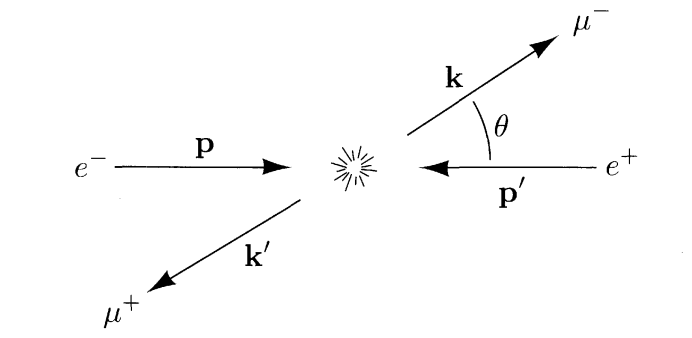
\includegraphics[width=0.6\textwidth]{trailer.png}
\caption{\label{trailer}\emph{electron positron annihilation}}
\end{figure}


\item The calculation we would like to perform is the differential cross section, that is the derivative of the cross section $\sigma$ with respect to the solid angle $\Omega$, $\frac{d \sigma}{d \Omega}$. This is a useful quantity as it is easily experimentally observed. In a particle collider, electrons and positrons are prepared in batches of length $l_A$ and $l_B$ and densities $\rho_A$ and $\rho_B$ respectively. When the two batches collide if the over lapping area of the head on collision is A, then the cross section is given by:
\end{itemize}

\begin{equation*}
  \sigma = \frac{\text{Number of events}}{\rho_A\rho_B l_A l_B A}
\end{equation*}

\begin{itemize}
  \item We now look at the dimensions of our quantities. Conveniently from our use of God given units, i.e. $\hbar =c =1$ we have that momentum, mass and energy have the same units as the energy mass equivalence becomes $E^2 = p^2 + m^2$. We also have from the Heisenberg's uncertainty principle that $\Delta p \Delta x \sim 1$. Thus the dimensions of mass and length are inversely related. 

  We can from this easily see that the dimensions of the quantity $[\rho_A\rho_B l_A l_B A]$ is $[m^2]$, which makes the dimensions of $\left[\frac{d\sigma}{d \Omega}\right] = \left[\frac{1}{m^2}\right]$ as angles are unitless. With this we can say that this quantity is also inversely proportional to the energy squared times some positive quantity that depends on the angle:


\begin{flalign}
\label{diff_cross}
  \frac{d\sigma}{d \Omega} \propto \frac{1}{E^2}|\mathcal{M}(\theta)|^2 
\end{flalign}
Here $\mathcal{M}$ is a dimensionless quantity, that is essentially the quantum mechanical amplitude for the process to occur. It does not depend on the energy $E$, as we are considering the limit where $E >> m_e,m_{\mu}$. This means we are unable to construct any dimensionless quantity like $E/m_e$ or $E/m_{\mu}$ as we have set $m_e/E = 0 = m_{\mu}/e$. Note that we could not take this limit and them $\mathcal{M}$ would depend on $E$, but it is simpler to consider the high energy limit. We will later calculate what the constant of proportionality in this equation is, and it turn out to be $1/64\pi^2$.
\end{itemize}
\begin{itemize}
  \item If we recall from Quantum mechanics, in perturbation theory we had that at first order the transition amplitude is related to the initial and final states along with the interaction Hamiltonian $H_i$, so:

\begin{equation*}
  \mathcal{M} \sim \bra{\text{final state}} H_I \ket{\text{initial state}}
\end{equation*}
But we know physically that the electrons do not interact with the muons, Instead what we know happens is that the electrons annihilate to form photons which in turn form the muons. This then means that $\bra{\mu^+ \mu^-} H_I \ket{e^+e^-} = 0 $ and instead we have that:

\begin{flalign}
\label{second order M}
  \mathcal{M} \sim \bra{\mu^+ \mu^-} H_I \ket{\gamma}^{\alpha}\bra{\gamma}H_I\ket{e^+e^-}_{\alpha}
\end{flalign}

This is a heuristic way of writing this second order contribution, but it makes sense physically as we have the electron positron pair interacting to become a photon ($\ket{\gamma}\bra{\gamma}$) and then the photon in turn becoming muons. Note the addition of vector indices ($\alpha$) as the photon is a vector particle (non-zero spin), so the photon created has 4 intermediate states, 3 for spin as it has spin-1 and one extra that comes from the fact that we are adding angular momenta in the four dimensional Lorentz group and must consider boosts also. (Remember the three spin components are generated by the three angular momentum operators and there is a corresponding generator for boosts). 
\end{itemize}

\begin{itemize}

  \item Since the photon must conserve angular momentum going to or from either of the two particles, the photon vector must be in the same direction as the axes of the particle pairs. We also know that the strength of the coupling between electrons (or muons) and photons is given by the electric charge $e$. This means for the case where electron has spin up along x axis, the positron has spin down:
\begin{equation*}
  \bra{\gamma} H_I \ket{e^+ e^-}^{\alpha} \propto e(0,1,i,0)
\end{equation*}
And if we have the same for muon and anti-muon:
\begin{equation*}
  \bra{\gamma} H_I \ket{\mu^+ \mu^-}^{\alpha} \propto e(0,\cos{\theta},i,-\sin(\theta))
\end{equation*}

The vectors here have the first component as the time component and the last three are part of the the polarization vector of the photon. See Jackson third edition page 299 for these vectors. 


\item When considering the experimental calculation of $\frac{d\sigma}{d \Omega}$ it also easier to account for all possible initial and final spin states, for which we need to take in to account conservation of angular momentum. This means we cant have two right polarized electron and positrons going to a left and right polarized muon and anti-muon. This condition then leaves 4 possible transitions which we can calculate the contributions. These calculations are done by dotting the two vectors we have above as in \ref{second order M}, making sure to take the complex conjugate of the first 4 vector and also remember to properly contract with the $(+---)$ metric. This results in:

\begin{flalign*}
& M(RL \rightarrow RL) \sim -e^2(1+\cos{\theta}) \\
& M(RL \rightarrow LR) \sim -e^2(1-\cos{\theta}) \\
& M(LR \rightarrow RL) \sim -e^2(1-\cos{\theta}) \\
& M(LR \rightarrow LR) \sim -e^2(1+\cos{\theta})
\end{flalign*}


There are no states that have 0 total angular momentum before and after as it turn out the intermediate photon (despite being a spin-1 boson) cant have spin 0 along an axis. Though in this case we would be requiring that the photon would have 0 total spin which is also not possible. 


\item We can finally take these 4 probabilities and square and sum them to get $|\mathcal{M}|^2$. Resulting in:

\begin{equation*}
  |\mathcal{M}|^2 \sim 4e^2(1+\cos^2{\theta})
\end{equation*}
So using \ref{diff_cross} and its proportionality constant $1/64\pi^2$ we can write:

\begin{equation*}
  \frac{d \sigma}{d \Omega} = \frac{e^2}{32E^2}(1+\cos^2{\theta})
\end{equation*}
Defining the constant $\alpha = e^2/4\pi \sim 137^{-1}$, we can then integrate this to get a expression for the total cross section as:

\begin{flalign*}
  \sigma = \frac{4\alpha^2\pi}{3E^2}
\end{flalign*}
This is the correct first order approximation!
\end{itemize}


\newpage  

\section{The need for Fields}
In this section we will see where regular quantum mechanics fails and what we need to do to fix it. 

\subsection{Non-relativistic free particle}

\begin{itemize}
  \item We can recall from QM that the probability of a particle at point $x$ at time $t$ propagating to $x'$ at time $t'$ is given by:
  \begin{equation}
  \label{propagator}
    \bra{x} e^{-iH(t-t')} \ket{x'}
  \end{equation}
  Here $H$ is the Hamiltonian. For a Non-relativistic free particle we have that $H = \hat{\textbf{P}}^2/2m$. We can then go about solving dor this propagator with this Hamiltonian in the usual way. This involves inserting the identity $\int \frac{d^3p}{(2\pi)^3}\ket{p}\bra{p} = \mathbb{I}$ into the above propagator \ref{propagator}before the $\ket{x'}$

  \begin{equation*}
      \bra{x} e^{-iH(t-t')} \ket{x'}  = \int \frac{d^3p}{(2\pi)^3}\bra{x}e^{-i\frac{\hat{\textbf{P}}^2}{2m}(t-t')}\ket{p}\braket{p|x'}
  \end{equation*}
  Then if we recall that $\braket{p|x'} = e^{-i\textbf{p}\cdot\textbf{x}'}$, $\braket{x|p} = e^{i\textbf{p}\cdot\textbf{x}}$ and $e^{-i\frac{\hat{\textbf{P}}^2}{2m}(t-t')}\ket{p} = e^{-i\frac{p^2}{2m}(t-t')}\ket{p}$. We get:

  \begin{flalign*}
    \bra{x} e^{-iH(t-t')} \ket{x'} & = \int \frac{d^3p}{(2\pi)^3}e^{-i\frac{p^2}{2m}(t-t')}e^{i\textbf{p}\cdot(\textbf{x}-\textbf{x}')} \\
    & = \left(\frac{m}{2\pi i(t-t')}\right)^{3/2}e^{im\frac{(\textbf{x}-\textbf{x}')^2}{2(t-t')}}
  \end{flalign*}
  \item What this is saying, is that for any two points $x$ and $x'$, no matter how far they are separated, have a non-zero probability of propagation from one to another. But this is direct contrast with what we know from special relativity! Two points separated by enough distance so that there space time interval, $\Delta s^2 = (t-t')^2 -|\textbf{x}-\textbf{x}'|^2$ is negative, i.e. space like. Which would require a propagation speed faster then light. 
\end{itemize}
\subsubsection{Non-trivial Gaussian integral}
\begin{itemize}
  \item In the above calculation we have to evaluate the following integral: 
  \begin{align*}
    \int_{\infty}^{\infty}e^{-(p+ia)^2}dp 
  \end{align*}
  Now we may think we can just make the substitution $u=p+ia$, but since we are involving complex numbers, we get a non trivial problem with the limits, as they change to $\infty-ia$ and $\infty+ia$. What we can do instead is calculate the integral of a closed contour. Since the integrand above has no poles, we know that any closed contour on the complex plain should evaluate to 0. What we will do is then modify the limits of our integral to be from $-q$ to $q$, we will take the limit at the end to recover what we got. We can then integrate along the following path: We start at $q+ia$ and move to $-q+ia$, then from $-q+ia$ to $-q$, from  $-q$ to $q$ and from $q$ to $q+ia$. This is a closed contour, that we will call $C$. We then have that:
  \begin{align*}
        0=\int_{C}e^{-z^2}dz = \int_{q+ia}^{-q+ia}e^{-(x)^2}dx+\int_{a}^{0}e^{-(-q+iy)^2}dy+\int_{-q}^{q}e^{-x^2}dx+\int_{0}^{a}e^{-(q+iy)^2}dy
     \end{align*}  
     We can then immediately argue that the second and fourth integrals should vanish when we send $q$ to infinity. Then the first integral we can reverse the limits and pick up a minus sign so: 
     \begin{align*}
        \int_{-q+ia}^{q+ia}e^{-(x)^2}dx = \int_{-q}^{q}e^{-x^2}dx = \sqrt{\pi}
      \end{align*} 
      And then finally now we can make a $u$-substitution of the LHS, to get back our original integral! So we can see in this case that since the two ends of this contour vanished in the arge $q$ limit we are essentially able to move our contour up and down to get the regular Gaussian integral.  
\end{itemize}

\subsection*{Relativistic free particle}
\begin{itemize}
  \item But we can chalk this up to a mistake. We were not considering the Hamiltonian of a \textbf{relativistic} free particle. That is, with the Hamiltonian $H  = \sqrt{\textbf{P}^2 + m^2}$. The propagator in a similar manner to before then becomes: 
  \begin{equation*}
  \begin{split}
     \bra{x} e^{-i\sqrt{\textbf{P}^2 + m^2}(t-t')} \ket{x'} & = \int \braket{x|p}  e^{-i\sqrt{\textbf{P}^2 + m^2}(t-t')}  \braket{p|x'}\frac{d^3p}{(2\pi)^3} \\
     & = \int \frac{d^3p}{(2\pi)^3}  e^{-i\sqrt{p^2 + m^2}(t-t')+ i\textbf{p}\cdot(\textbf{x}-\textbf{x}')} 
  \end{split}
  \end{equation*}
  We can then parametrize the angle part of this integral by letting $\theta$ be the angle between $\textbf{p}$ and $(\textbf{x}-\textbf{x}')$, we can also further parametrize this with $\eta = \cos{\theta}$:
  \begin{equation*}
  \begin{split}
  \bra{x} e^{-i\sqrt{\hat{\textbf{P}}^2 + m^2}(t-t')} &\ket{x'}  = \int_{0}^{\infty} \frac{p^2dp}{(2\pi)^2}  \int_{-1}^{1} d \eta e^{-i\sqrt{p^2 + m^2}(t-t')+ ip|\textbf{x}-\textbf{x}'|\eta} \\
   = \int_{0}^{\infty} \frac{p^2dp}{(2\pi)^2}& e^{-i\sqrt{p^2 + m^2}(t-t')} \frac{1}{ip|\textbf{x}- \textbf{x}'|}\left(e^{ ip|\textbf{x}-\textbf{x}'|}-e^{- ip|\textbf{x}-\textbf{x}'|} \right)
  \end{split}
  \end{equation*}
  We can then turn this into an integral from $-\infty$ to $\infty$ with a factor of 2:
  \begin{equation}
  \label{Rel_propagator}
  \begin{split}
 = \frac{-i}{2\pi^2|\textbf{x}- \textbf{x}'|}\int_{0}^{\infty}pdp~e^{-i\sqrt{p^2 + m^2}(t-t')+ip|\textbf{x}-\textbf{x}'|}
  \end{split}
  \end{equation}
\end{itemize}
\subsubsection{Laplace steepest decent}
\begin{itemize}
  \item We can then use a useful approximation of integrals of this form by expanding around critical points. That is points $x_0$ where $f'(x_0)= 0$. The approximation is as follows, for a critical point $x_0$ of $f(x)$:
  \begin{flalign*}
\int_{-\infty}^{\infty}&h(x)e^{Af(x)}dx =  \int_{-\infty}^{\infty}h(x)e^{A\left[f(x_0) + \frac{1}{2}f''(x_0)(x-x_0)^2+\mathcal{O}((x-x_0)^3)\right]}dx \\ 
 \approx   h(x_0)e^{Af(x_0)}&\int_{-\infty}^{\infty}e^{-A\frac{1}{2}|f''(x_0)|(x-x_0)^2}dx = \sqrt{\frac{2\pi}{A|f''(x_0)|}}h(x_0)e^{Af(x_0)} 
  \end{flalign*}
  \item Where we have assumed $x_0$ is a global maxima so that $f''(x_0) \leq 0$. This approximation works well as the exponential ensures that any small deviation from $x_0$ contributes very little to the integral. It of course depends also on $h(x)$ being "well behaved".


  \item Back to the relevant integral \ref{Rel_propagator}, we can see that for us $f(p) = -i\sqrt{p^2 + m^2}(t-t')+ip|\textbf{x}-\textbf{x}'|$ and $h(p) = p$. So we find the stationary point of $f(p)$ via $f'(p_0)=0$: 
  \begin{equation*}
  \begin{split}
      f'(p_0) = \frac{-p_0(t-t')}{\sqrt{p_0^2+m^2}}+|\textbf{x}-\textbf{x}'| =0 \implies p_0^2 = \frac{m^2|\textbf{x}-\textbf{x}'|^2}{(t-t')^2-|\textbf{x}-\textbf{x}'|^2}
      \end{split}
    \end{equation*}  
    Then we can evaluate $f(p_0)$:
    \begin{equation*}
    \begin{split}
      f(p_0) & = -i\sqrt{\frac{m^2|\textbf{x}-\textbf{x}'|^2}{(t-t')^2-|\textbf{x}-\textbf{x}'|^2}+m^2}(t-t')+i\sqrt{\frac{m^2|\textbf{x}-\textbf{x}'|^2}{(t-t')^2-|\textbf{x}-\textbf{x}'|^2}} \\
      & = -\frac{m(|\textbf{x}-\textbf{x}'|^2-(t-t')^2)}{\sqrt{|\textbf{x}-\textbf{x}'|^2-(t-t')^2}} = -m\sqrt{|\textbf{x}-\textbf{x}'|^2-(t-t')^2}
    \end{split}
    \end{equation*}
    Where we have used the fact that we are considering probabilities outside the light-cone, i.e. where $|\textbf{x}-\textbf{x}'| > (t-t')$, so that the square root $ \sqrt{(t-t')^2-|\textbf{x}-\textbf{x}'|^2}=i\sqrt{|\textbf{x}-\textbf{x}'|^2-(t-t')^2}$ . 

    \item With this we can now use Laplace's steepest decent integral approximation to write:
    \begin{flalign*}
    \bra{x} e^{-i\sqrt{\hat{\textbf{P}}^2 + m^2}(t-t')} \ket{x'} \propto h(p_0)e^{f(p_0)} \propto e^{-\sqrt{|\textbf{x}-\textbf{x}'|^2-(t-t')^2}}
    \end{flalign*}
    This again does not solve our problem, we have that there is a non-zero probability of propagating to outside the light-cone. Some more radical approach is needed to solve this problem. 
\end{itemize}

\subsection{Field theory EoM}
\begin{itemize}
  \item The  Idea will be to go from dealing with particle, to waves. For this we need to generalize our idea of action being the integral of a Lagrangian over time to being the integral of a Lagrange density over time and space as a field is spread out, not localized. This means:
  \begin{equation*}
    S = \int L(q_i,\dot{q}_i,t)dt \rightarrow \int d^4x\mathcal{L}(\varphi(\textbf{x},t),\partial_{\mu} \varphi(\textbf{x},t))
  \end{equation*}
  We then have to vary this action to set $\delta S = 0$:
  \begin{equation*}
    \delta S = \int d^4x \left(\frac{\delta \mathcal{L}}{\delta \varphi}\delta \varphi  - \frac{\delta \mathcal{L}}{\delta \partial_{\mu} \varphi}\delta\partial_{\mu}\varphi\right) = \int d^4x \left(\frac{\delta \mathcal{L}}{\delta \varphi}  - \partial_{\mu}\left(\frac{\delta \mathcal{L}}{\delta \partial_{\mu} \varphi}\right)\right)\delta \varphi 
  \end{equation*}
  \begin{flalign}
  \label{EoM}
    \implies \frac{\delta \mathcal{L}}{\delta \varphi}  - \partial_{\mu}\frac{\delta \mathcal{L}}{\delta \partial_{\mu} \varphi} = 0 
  \end{flalign}
  Where we have integrated by parts the second term.
\end{itemize}

\subsection{Non-degenerate Lagrangian}
\begin{itemize}
  \item It is often the case, that when we have constructed our Lagrangian, that we would like to perform a Legendre transform from the variables $q$ and $\dot{q}$, to $q$ and $p$. This is gives us our Hamiltonian and takes the form $H =\sum_i p_i \dot{q}_i  - L(q,\dot{q})$. In doing this we are required to solve for $\dot{q}$ in terms of $q$ and $p$. But this is not always possible, for example given the Lagrangian $L \propto \dot{q} \implies p = \frac{\partial L}{\partial q} = 1$, so we are unable to solve for $\dot{q}(p,q)$. It turn out the condition for us to always be able to solve for $\dot{q}$ is as follows:

  If we denote the matrix $M_{ij} = \frac{\partial^2 L}{\partial\dot{q}^i\partial\dot{q}^j}$, then the condition becomes, we can solve for $\dot{q}_{i} \iff \text{det}(M) \neq 0$. The Lagrangian can then be written as:

  \begin{equation*}
  L = \sum_{i,j}M_{ij}\partial\dot{q}^i\partial\dot{q}^j, ~~~ \text{and}~~~ \dot{q}^i  = \sum_{j}M^{-1}_{ij}p_j
  \end{equation*}
  This is called a Non-degenerate Lagrangian. 
\end{itemize}

\subsection{Hamiltonian field theory} 
\begin{itemize}
  \item We wish to find a Hamiltonian for our field theory. The best way to go about extending our definition of $H =\sum_i p_i \dot{q}_i  - L(q,\dot{q})$, is to think of space as a discretized space, as we had the co-ordinates $q$ indexed by $i$. We can then calculate:

  \begin{equation*}
  p(\textbf{x}) = \frac{\partial L}{\partial \dot{\phi}} = \frac{\partial }{\partial \dot{\phi}(\textbf{x})}\sum_{\textbf{y}}\mathcal{L}(\phi(\textbf{y}),\dot{\phi}(\textbf{y}))d^3y = \pi(\textbf{x})d^3x. 
  \end{equation*}
  Where:
  \begin{flalign}
  \label{pi}
  \pi(\textbf{x}) = \frac{\partial \mathcal{L}}{\partial \dot{\phi}(\textbf{x})}
  \end{flalign}
  This is called the \emph{momentum density} conjugate to $\phi(\textbf{x})$. We can now write the Hamiltonian as:
  \begin{equation*}
    H = \sum_{\textbf{x}}p(\textbf{x})\dot{\phi}(\textbf{x}) - L
  \end{equation*}
  Which in the continuum limit becomes:
  \begin{flalign}
\label{Hamiltonian}
     H = \int d^3x[\pi(\textbf{x})\dot{\phi}(\textbf{x}) - \mathcal{L}] \equiv \int d^3x\mathcal{H} 
   \end{flalign} 
\end{itemize}


\subsection{Noether's Theorem}
\begin{itemize}
  \item We are used to Noether's Theorems relation between symmetries and conservation in the context of particles. We will now discuss this in the context of fields. If we have an infinitesimal transformation of fields taking the form:
  \begin{equation*}
     \phi(x) \rightarrow \phi'(x) = \phi(x) + \alpha\Delta\phi(x)
   \end{equation*} 
Here $\alpha$ is small. This transformation is a symmetry if it results in the same EoM, i.e. leaves the action unchanged. This means the Lagrangian must be the same up to the addition of a total derivative, which in this context is the 4-gradient:
\[
      \mathcal{L}(x) \rightarrow \mathcal{L}(x) + \alpha \partial_{\mu}\mathcal{J}^{\mu}(x)
\]
    Where $\mathcal{J}^{\mu}$ is some 4-vector. We can then find the expected form of $\Delta \mathcal{L}(\phi,\partial_{\mu}\phi )$:
    \begin{align*}
     \alpha \Delta \mathcal{L} & = \frac{\partial \mathcal{L}}{\partial \phi}(\alpha \Delta \phi) + \left(\frac{\partial \mathcal{L}}{\partial (\partial_{\mu}\phi)}\right)\partial_{\mu}(\alpha\Delta\phi) \\
    &  = \alpha \partial_{\mu}\left(\frac{\partial \mathcal{L}}{\partial(\partial_{\mu}\phi)}\Delta \phi\right)+\alpha\left[\frac{\partial\mathcal{L}}{\partial \phi} - \partial_{\mu}\left(\frac{\partial \mathcal{L}}{\partial(\partial_{\mu}\phi)}\right)\right]\Delta \phi 
    \end{align*}
    We can then recognize that the second term vanished via our EoM \ref{EoM}, so we can set the remaining term to $\alpha \partial_{\mu}\mathcal{J}^{\mu}(x)$, which is equivalent to:
\begin{flalign}
\label{Noether}
  \partial_{\mu}j^{\mu}(x) = 0, ~~~~\text{for} ~~j^{\mu}(x) = \frac{\partial \mathcal{L}}{\partial(\partial_{\mu}\phi)}\Delta \phi - \mathcal{J}^{\mu}
\end{flalign}
\item If the symmetry involves more then one field the first term above should be a sum of those terms, for the different fields. This conservation law also implies that there is a charge constant in time namely:
\begin{flalign*}
Q \equiv \int j^{0} d^3x
\end{flalign*}
\end{itemize}
\subsection{Stress-Energy Tensor}
\begin{itemize}
\item We can also consider transformations of space itself, for example, translations or rotations. This takes the for $x^{\mu} \rightarrow x^{\mu} - a^{\mu}$, which has the following affect on the fields (when infinitesimal): 

\[ 
  \phi(x) \rightarrow \phi(x+a) = \phi(x) + a^{\mu}\partial_{\mu}\phi(x)
 \]
The Lagrangian must also transform in the same way as it is also a scalar:
\[ 
  \mathcal{L}(x) \rightarrow \mathcal{L}(x+a) = \mathcal{L}(x) + a^{\nu}\partial_{\mu}(\delta^{\mu}_{\nu}\mathcal{L}(x))
 \]
 We can then recognize the $\delta^{\mu}_{\nu}\mathcal{L}(x)$ as $ \sim \mathcal{J}^{\mu}$ from \ref{Noether}, however since the change in the scalar field became a vector $\Delta \phi \rightarrow \partial_{\mu}\phi(x)$, then we must add a second index to our $\mathcal{J}^{\mu} \rightarrow \mathcal{J}^{\mu}_{~\nu}$. This is for the reason for the $\delta_{\nu}^{\mu}$ in the above expression and means our conserved vector $j^{\mu}$ becomes a conserved tensor of the form:

 \begin{flalign*}
      \partial_{\mu}T^{\mu}_{~\nu}(x) = 0, ~~~~\text{for} ~~T^{\mu}_{~\nu}(x) = \frac{\partial \mathcal{L}}{\partial(\partial_{\mu}\phi)}\partial_{\nu}\phi - \delta^{\mu}_{\nu}\mathcal{L}
  \end{flalign*} 
  This is the \emph{Stress-Energy Tensor} also called the \emph{Energy-Momentum Tensor}. We can then notice that the conserved charge associated with the time translations is nothing more then out Hamiltonian:
  \[
\int T^{00}d^3x = \int\left(\frac{\partial \mathcal{L}}{\partial\dot{\phi}}\dot{\phi} - \mathcal{L}\right)d^3x = \int \mathcal{H}d^3x = H  
  \] 
  Similarly for space translation the conserved charges are the physical momenta, not to be confused with the canonical momentum.
  \[  
  \int T^{0i}d^3x = \int \mathcal{P}_id^3x = P_i 
  \] 
\end{itemize}
\newpage
\section{The Klein-Gordon Field}
\begin{itemize}
  \item We ease ourselves into the concepts of quantum fields with the discussion of the Klein-Gordon field. This is one of the simplest types of fields and its use becomes obvious when we see the EoM, which is just the Schr\"odinger equation but made relativistic by replacing $\hat{\textbf{p}}^2/2m \rightarrow \sqrt{\hat{\textbf{p}}^2 + m^2}$. We will see more of this later.

     \item The Lagrange density for the Klein-Gordon field takes the form:
     \begin{equation}
       \label{KG field}
       \mathcal{L} = \frac{1}{2}\partial_{\mu} \phi \partial^{\mu}\phi -\frac{m^2}{2}\phi^2
     \end{equation}   
From this we can calculate the momentum density via \ref{pi} to get $\pi = \dot{\phi}$. And thus via \ref{Hamiltonian} the Hamiltonian density is:
\begin{equation}
\label{KG_Ham}
  \mathcal{H} = \frac{1}{2}\left(\pi^2 +(\nabla\phi)^2+m^2\phi^2\right) 
\end{equation}
\item The equations of motion can also be calculated easily via \ref{EoM} resulting in the \emph{Klein-Gordon equation}:
\begin{flalign}
\label{KG eq}
  (\partial_{\mu}\partial^{\mu}+m^2)\phi  = 0
\end{flalign} 
This $\partial_{\mu}\partial^{\mu}$ is often denoted $\Box$. As an aside, if we "make" the Schr\"odinger equation relativistic, i.e. $\textbf{p}^2 + m^2 = E^2$ and use the definition of the operators $ i\partial_t\psi= E\psi $ and $\hat{\textbf{p}} = -i\nabla$, so:  $-\nabla^2 + m^2 = -\partial^2_t$, recovering us the above Klein-Gordon equation.  
\end{itemize}

\subsection{Second Quantization}
\begin{itemize}
  \item We will now see if we can ``quantize'' this field. What we can do to help figure out how to do this is to take inspiration from the quantization of the single particle Harmonic oscillator in QM. This works nicely as we can see the Lagrangian density for the Klein-Gordon field \ref{KG field} resembles that of the harmonic oscillator. By quantize here we mean to reinterpret the dynamical variables as operators that obey canonical commutation relations, like $[p_i,q_j] = i\delta_{i,j},~[q_i,q_j] = 0 = [p_i,p_j]$. Instead however $\phi$ and $\pi$ will become our operators and we will require that $[\phi(\textbf{x}),\pi(\textbf{y})] = i \delta(\textbf{x}-\textbf{y}),~ [\phi(\textbf{x}),\phi(\textbf{y})] = 0 = [\pi(\textbf{x}),\pi(\textbf{y})]$. This procedure is often called \emph{Second Quantization} to distinguish it from the old one particle version. 
  
  \item Our goal is to now find the spectrum of the Hamiltonian. We start by taking our field $\phi(\textbf{x})$ and writing it in terms of its Fourier transform to momentum (p)-space
\[
  \phi(\textbf{x}) = \int \frac{d^3p}{(2\pi)^3}\phi(\textbf{p})e^{i\textbf{p}\cdot\textbf{x}}
\]
Here we also require that $\phi(\textbf{x},t)$ is real so $\phi^{\ast}(\textbf{p}) = \phi(-\textbf{p})$ Then using the Klein-Gordon equation \ref{KG eq} we get the condition:
\[
  \left[\partial_t^2 + p^2+m^2\right]\phi(\textbf{p}) = 0 
\]
Where we have acted the $-\partial^2_{i}$ from $\Box$ on the exponential to pull out the $p^2$ This equation of motion is the same as that of a harmonic oscillator with frequency $\omega_{\textbf{p}} = \sqrt{p^2+m^2}$. 

\item We now recall from QM that in order to solve the harmonic oscillator we introduced the creation ($\hat{a}^{\dagger}$) and annihilation ($\hat{a}$) operators, so that we could write $\hat{q} = \frac{1}{\sqrt{2 \omega}}(\hat{a}+\hat{a}^{\dagger})$ and $\hat{p} = -i\sqrt{\frac{\omega}{2}}(\hat{a}-\hat{a}^{\dagger})$. This then meant the Hamiltonian took the form $H = \frac{1}{2}(\hat{p}^2+\omega^2\hat{q}^2) = \omega(\hat{a}^{\dagger}\hat{a}+\frac{1}{2})$ and also that the commutators  were: $[H,\hat{a}^{\dagger}] = \omega \hat{a}^{\dagger}$ , $[H,\hat{a}] = -\omega \hat{a}$ and $[a,a^{\dagger}] =\mathcal{I}$. 
 
\item This can be done for our field $\phi$, except we have to consider that $\hat{q} = \frac{1}{\sqrt{2 \omega}}(\hat{a}+\hat{a}^{\dagger})$ is a function of momentum as for us we have $\omega_{\textbf{p}} = \sqrt{p^2+m^2}$. We can then recall that since we expect $\phi$ to be real we require that $\phi^{\dagger}(\textbf{p}) = \phi(-\textbf{p})$, this means we should have $\phi(\textbf{p}) \propto a_{\textbf{p}}+a^{\dagger}_{-\textbf{p}}$ as then $\phi(\textbf{p})^{\dagger} \propto a_{\textbf{p}}^{\dagger}+ a_{-\textbf{p}} \propto \phi(-\textbf{p})$. This means our corresponding expression for $\phi$ should take the form:
\begin{equation}
\label{phi_1}
  \phi(\textbf{x}) = \int \frac{d^3p}{(2\pi)^3}\frac{1}{\sqrt{2\omega_{\textbf{p}}}}\left(a_{\textbf{p}}+a^{\dagger}_{-\textbf{p}}\right)e^{i\textbf{p}\cdot\textbf{x}} 
\end{equation} 
\begin{equation}
\label{pi_1}
  \pi(\textbf{x}) = -i\int \frac{d^3p}{(2\pi)^3}\sqrt{\frac{\omega_{\textbf{p}}}{2}}\left(a_{\textbf{p}}-a^{\dagger}_{-\textbf{p}}\right)e^{i\textbf{p}\cdot\textbf{x}} 
\end{equation} 
We can also think of this expression as each Fourier mode of the field being treated as an independent oscillator with its own $a$ and $a^{\dagger}$ (which will also be a function of the momentum). We can then isolate the second term in this integral and change $\textbf{p}$ to $-\textbf{p}$, since we are integrating over all momentum space, this just results in the signs of the $p$'s in the term changing so we can write:

\begin{flalign}
\label{phi_2}
  \phi(\textbf{x}) = \int \frac{d^3p}{(2\pi)^3}\frac{1}{\sqrt{2\omega_{\textbf{p}}}}\left(a_{\textbf{p}}e^{i\textbf{p}\cdot\textbf{x}}+a^{\dagger}_{\textbf{p}}e^{-i\textbf{p}\cdot\textbf{x}}\right) 
\end{flalign}
In a similar manner the momentum density can be written as:

\begin{flalign}
\label{pi_2}
  \pi(\textbf{x}) = -i\int \frac{d^3p}{(2\pi)^3}\sqrt{\frac{\omega_{\textbf{p}}}{2}}\left(a_{\textbf{p}}e^{i\textbf{p}\cdot\textbf{x}}-a^{\dagger}_{\textbf{p}}e^{-i\textbf{p}\cdot\textbf{x}}\right) 
\end{flalign}
\end{itemize}
\subsubsection{Commutators}
\begin{itemize}
\item We can then go about checking the commutator $[\phi(\textbf{x}),\pi(\textbf{x}')]= i \delta(\textbf{x}-\textbf{y})$ which should be equivalent to the the new creation and annihilation operators satisfying $[a,a^{\dagger}] = (2 \pi)^{3}\delta(\textbf{p}-\textbf{p}')$. Using the above definitions \ref{phi_1} and \ref{pi_1} for this calculation is easier, resulting in:
\begin{equation}
\begin{split}
  [\phi(\textbf{x}),\pi(\textbf{x}')] & = -\frac{i}{2}\int \frac{d^3pd^3p'}{(2\pi)^6}\sqrt{\frac{\omega_{\textbf{p}'}}{\omega_{\textbf{p}}}}\left[-a_{\textbf{p}}a^{\dagger}_{\textbf{-p}'} + a^{\dagger}_{\textbf{-p}}a_{\textbf{p}'}-(-a^{\dagger}_{\textbf{p}'}a_{\textbf{-p}} + a_{\textbf{p}}a^{\dagger}_{\textbf{-p}'})\right]e^{i(\textbf{p}\cdot \textbf{x}+\textbf{p}'\cdot \textbf{x}')} \\ 
  &  = -\frac{i}{2}\int \frac{d^3pd^3p'}{(2\pi)^6}\sqrt{\frac{\omega_{\textbf{p}'}}{\omega_{\textbf{p}}}}\left[[a^{\dagger}_{\textbf{-p}},a_{\textbf{-p}'}]-[a_{\textbf{p}},a^{\dagger}_{\textbf{-p}'}]\right]e^{i(\textbf{p}\cdot \textbf{x}+\textbf{p}'\cdot \textbf{x}')}  \\ 
   & =  -\frac{i}{2}\int \frac{d^3pd^3p'}{(2\pi)^6}\sqrt{\frac{\omega_{\textbf{p}'}}{\omega_{\textbf{p}}}}(2\pi)^3\left[-\delta(\textbf{p}'+\textbf{p}) -\delta(\textbf{p}+\textbf{p}') \right]e^{i(\textbf{p}\cdot \textbf{x}+\textbf{p}'\cdot \textbf{x}')}  \\ 
   & = i\int \frac{d^3p}{(2\pi)^3}e^{i\textbf{p}\cdot( \textbf{x} -\textbf{x}')} = i\delta(\textbf{x} -\textbf{x}')  
  \end{split}
  \end{equation}  
  Where we have used the fact that $\omega_{\textbf{p}}=\omega_{\textbf{-p}}$ by definition. We can then also calculate the Hamiltonian via \ref{KG_Ham}:
  \begin{equation*}
    \begin{split}
      H  = \frac{1}{2}\int &d^3x\int\frac{d^3pd^3p'}{(2\pi)^6}\left[\frac{-\sqrt{\omega_{\textbf{p}}\omega_{\textbf{p}'}}}{2}\left(a_{\textbf{p}}-a^{\dagger}_{\textbf{-p}}\right)\left(a_{\textbf{p}'}-a^{\dagger}_{\textbf{-p}'}\right)\right. \\
       & \left. + \frac{-\textbf{p}\cdot \textbf{p}'+m^2}{2\sqrt{\omega_{\textbf{p}}\omega_{\textbf{p}'}}}\left(a_{\textbf{p}}+a^{\dagger}_{\textbf{-p}}\right)\left(a_{\textbf{p}'}+a^{\dagger}_{\textbf{-p}'}\right)\right]e^{i\textbf{x}\cdot(\textbf{p}+\textbf{p}')} \\
    \end{split}
  \end{equation*}
  We can then notice that the $\textbf{x}$ part of this integral creates a delta function $\int d^3xe^{i\textbf{x}\cdot(\textbf{p}+\textbf{p}')} = (2\pi)^{3}\delta(\textbf{p}+\textbf{p}')$, so $\textbf{p}= - \textbf{p}'$. This allows us to write:
  \begin{equation*}
    \begin{split}
    H  & = \frac{1}{4}\int\frac{d^3p}{(2\pi)^3}\omega_{\textbf{p}}\left[-\left(a_{\textbf{p}}-a^{\dagger}_{\textbf{-p}}\right)\left(a_{\textbf{-p}}-a^{\dagger}_{\textbf{p}}\right) + \left(a_{\textbf{p}}+a^{\dagger}_{\textbf{-p}}\right)\left(a_{\textbf{-p}}+a^{\dagger}_{\textbf{p}}\right) \right]  \\ 
    & = \frac{1}{2}\int\frac{d^3p}{(2\pi)^3}\omega_{\textbf{p}}\left[a_{\textbf{p}}a^{\dagger}_{\textbf{p}}+a^{\dagger}_{\textbf{-p}}a_{-\textbf{p}}\right]
 \end{split}
  \end{equation*}
  We can then for this second term do the same trick of changing $\textbf{p} \rightarrow -\textbf{p}$, which does not affect the integral's value as $\omega_{\textbf{p}} = \omega_{-\textbf{p}}$. Then also using the fact that $a^{\dagger}_{\textbf{p}}a_{\textbf{p}} = a_{\textbf{p}}a^{\dagger}_{\textbf{p}}-[a_{\textbf{p}},a^{\dagger}_{\textbf{p}}]$ we get the final result that:

  \begin{flalign}
  \label{Ham_SH}
  H = \int \frac{d^3p}{(2\pi)^3}\omega_{\textbf{p}}\left[a_{\textbf{p}}a^{\dagger}_{\textbf{p}}-\frac{1}{2}[a_{\textbf{p}},a^{\dagger}_{\textbf{p}}]\right]
  \end{flalign}
  If we stop to think about the second term in this expression we realize something strange, $[a_{\textbf{p}},a^{\dagger}_{\textbf{p}}] = (2\pi)^3\delta(0)$, which is and infinite constant (constant as in it wont affect any state we act $H$ on). But since this is constant we can never measure it experimentally as we only ever measure the energy shift between two different energies. We can also think of this as the zero point energy for each point in space, except that we made this space continuous resulting in infinite many oscillator ground states, so what did we expect really? This means we can ignore the second term in \ref{Ham_SH}.

   To make sure everything is consistent we also check the commutators, $[H,a_{\textbf{p}}^{\dagger}] = \omega a^{\dagger}_{\textbf{p}}$ , $[H,a_{\textbf{p}}] = -\omega a_{\textbf{p}}$:
   \begin{equation*}
      \begin{split}
        [H,a_{\textbf{p}}] & = \int \frac{d^3p'}{(2\pi)^3}\omega_{\textbf{p}'}\left[a_{\textbf{p}'}a^{\dagger}_{\textbf{p}'}a_{\textbf{p}}-a_{\textbf{p}}a^{\dagger}_{\textbf{p}'}a_{\textbf{p}'}\right] \\
        & = \int \frac{d^3p'}{(2\pi)^3}\omega_{\textbf{p}'}\left[a_{\textbf{p}'}a_{\textbf{p}}a^{\dagger}_{\textbf{p}'}-a_{\textbf{p}'}[a_{\textbf{p}},a^{\dagger}_{\textbf{p}'}]-a_{\textbf{p}}a_{\textbf{p}'}a^{\dagger}_{\textbf{p}'}\right] \\
        & = -\omega_{\textbf{p}}a_{\textbf{p}} 
      \end{split}
   \end{equation*}
   Here we have used the fact that $[a_{\textbf{p}},a_{\textbf{p}'}]= 0 = [a^{\dagger}_{\textbf{p}},a^{\dagger}_{\textbf{p}'}]$ to make the first and last term cancel. The commutator $[H,a^{\dagger}_{\textbf{p}}]=\omega_{\textbf{p}}a^{\dagger}_{\textbf{p}}$, can be calculated in the same manner.

   \item We can now start to think about the creation and annihilation operators as their name suggests. The ground state is $\ket{0}$ st. $a_{\textbf{p}}\ket{0} = 0$ and has $E=0$, where as acting with $a^{\dagger}_{\textbf{p}}$ increases the energy. These operators clearly depend on momentum $\textbf{p}$ so we can think of them as creating (and annihilating) momentum eigenstates. 
\end{itemize}

\subsection{Particle creation}
\begin{itemize}
\item The next step is to see if we can write out all the possible momentum states as powers of the creation operator $a^{\dagger}_{\textbf{p}}$. The question is then what is the choice of proportionality? We should of course have that the states are normalized, that is $\braket{\textbf{p}|\textbf{p}'} = \delta(\textbf{p}-\textbf{p}')$. This however, leads to a problem, namely that this quantity $\delta(\textbf{p}-\textbf{p}')$ is not Lorentz invariant. To see why, consider a boost along the $x_3$ direction. Using the property that $\delta(f(x)-f(x_0)) = \delta(x-x_0)/|f'(x_0)|$ we have that if we boost from momenta $\textbf{p},\textbf{p}' \rightarrow \tilde{\textbf{p}},\tilde{\textbf{p}}'$,so that $\tilde{p}_3 = \gamma(p_3+\beta E)$ and $\tilde{E} = \gamma(E + \beta p_3)$. Then we have that: 
\begin{equation*}
  \begin{split}
   &  \delta(\textbf{p}-\textbf{p}') = \delta(\tilde{\textbf{p}}-\tilde{\textbf{p}}') \frac{d \tilde{p}_3}{d p_3}  = \delta(\tilde{\textbf{p}}-\tilde{\textbf{p}}') \frac{d \gamma(p_3+\beta E)}{dp_3} \\
    &  =   \delta(\tilde{\textbf{p}}-\tilde{\textbf{p}}')\gamma \left(1 + \frac{d E}{dp_3}\right)  =  \delta(\tilde{\textbf{p}}-\tilde{\textbf{p}}')\frac{\gamma}{E} \left(E + \beta p_3\right) \\
    & =  \delta(\tilde{\textbf{p}}-\tilde{\textbf{p}}')\frac{\tilde{E}}{E} 
  \end{split}
\end{equation*}
Where we have used $E^2 = |\textbf{p}|^2+m^2$ to do the second last step. We can see from this that if we choose the normalization $\ket{\textbf{p}} = \sqrt{2E_{\textbf{p}}}(a^{\dagger}_{\textbf{p}}\ket{0}$ then $\braket{\textbf{p}|\textbf{p}'}$ is Lorentz invariant, as needed. 

\item With this we can consider the action of $\phi$ on the ground state $\ket{0}$. Via \ref{phi_2} this becomes: 

\[
  \phi(\textbf{x})\ket{0} = \int \frac{d^3p}{(2\pi)^3}\frac{1}{2E_{\textbf{p}}}e^{-i\textbf{p}\cdot \textbf{x}}\ket{\textbf{p}} 
\]
Where from here and now on we replace $\omega_{\textbf{p}}$ with $E_{\textbf{p}}$. This is similar to the Fourier expansion we have of $\ket{\textbf{x}}$ in regular QM, except for the factor of $1/E_{\textbf{p}}$, which is almost constant in the non-relativistic, so we can put forward the interpretation that the operator $\phi(\textbf{x})$ acting on the vacuum $\ket{0}$, creates a particle at position $\ket{\textbf{x}}$. 
\end{itemize}
\subsection{Time evolution}
\begin{itemize}
  \item We would now like to turn our heads to adding time evolution to our fields. So far we have been working in the Schr\"odinger picture and interpreted the resulting theory in terms of particles. We now switch to the Heisenberg picture where it is simpler to add time dependence. 

  We know the time evolution operator is a unitary operator $U(t)$, st. $\phi(x) = \phi(\textbf{x},t) = U^{\dagger}\phi(\textbf{x})U$. For a time independent Hamiltonian we just have the usual $U = e^{-iHt}$. If we want to calculate $\phi(x)$ we will need to know what $a(\textbf{p},t) = e^{iHt}a_{\textbf{p}}e^{-iHt}$ is. We know that $[H,a_{\textbf{p}}] = -E_{\textbf{p}}a_{\textbf{p}}$. So we can write:
  \begin{equation*}
  \begin{split}
  & Ha_{\textbf{p}} = [H,a_{\textbf{p}}]+a_{\textbf{p}}H = a_{\textbf{p}}(H-E_{\textbf{p}}) \\ 
  & \implies H^na_{\textbf{p}} = a_{\textbf{p}}(H-E_{\textbf{p}})^n
  \end{split} 
  \end{equation*}
  Where we can do the last step as $H$ commutes with both itself and $E_{\textbf{p}}$, so acting with further $H$'s from the left only yields more of the same factor. Similarly this means $H^na^{\dagger}_{\textbf{p}} = a^{\dagger}_{\textbf{p}}(H+E_{\textbf{p}})^n$. This then means that: 
\begin{align}
\label{a_H}
  e^{iHt}a_{\textbf{p}}e^{-iHt} = a_{\textbf{p}}e^{-iE_{\textbf{p}}t},~~~e^{iHt}a^{\dagger}_{\textbf{p}}e^{-iHt} = a^{\dagger}_{\textbf{p}}e^{-iE_{\textbf{p}}t}
\end{align}
  This means using \ref{phi_2} we can write $\phi(x)$ as:

  \begin{flalign}
  \label{phi_3}
  \phi(x) = \int \frac{d^3p}{(2\pi)^3}\frac{1}{\sqrt{2E_{\textbf{p}}}}\left(a_{\textbf{p}}e^{-ip^{\mu}x_{\mu}}+a^{\dagger}_{\textbf{p}}e^{ip^{\mu}x_{\mu}}\right) 
  \end{flalign}
  Where in the 4-vector (which we often just write as $p$ or $x$) $p_{0} = E_{\textbf{p}}$. 

  \item Peskin has the following nice interpretation of this equation: ``A positive-frequency solution of the field equation has as its coefficient the operator that \emph{destroys} a particle in that single-particle wavefunction. A negative-frequency solution of the field equation, being the Hermitian conjugate of a positive-frequency solution, has as its coefficient the operator that \emph{creates} a particle in that positive-energy single-particle wavefunction. In this way, the fact that relativistic wave equations have both positive- and negative-frequency solutions is reconciled with the requirement that a sensible quantum theory contain only positive excitation energies.'' 

  \item We can also use the Heisenberg equation of motion, which states that for an operator $\mathcal{O}$, $i\frac{\partial \mathcal{O}}{\partial t} = [\mathcal{O},H]$. This allows us to calculate $i\frac{\partial \phi(x)}{\partial t}$ as it must equal $[\phi(x),H]$, with $H$ given by \ref{KG_Ham}:
  \begin{equation*}
  \begin{split}
    i\frac{\partial \phi(x)}{\partial t} & = [\phi(x),\frac{1}{2}\int d^3x'\left(\pi^2(x') +(\nabla\phi(x'))^2+m^2\phi^2(x')\right) ] \\
      & =  \frac{1}{2}\int d^3x \left(\pi(x')[\phi(x), \pi(x')]+[\phi(x), \pi(x')]\pi(x') \right) \\
      & = i \pi(x)
  \end{split}
  \end{equation*}

\end{itemize}
\subsection{2-point correlation function}
\begin{itemize}
  \item  With all this formalism we now see if we can solve the problem of causality. That is, does $\braket{\textbf{x},\textbf{y}}$ vanish for $\textbf{y}$ outside the light cone. In the above formalism, $\braket{\textbf{x},\textbf{y}}$ takes the form $\bra{0}\phi(x)\phi(y)\ket{0}$. This is our propagator and will be denoted $D(x-y)$. We can use \ref{phi_3} to write this as:
  \begin{align*}
   D(x-y) & = \int \frac{d^3pd^3p'}{(2\pi)^6}\frac{1}{2\sqrt{E_{\textbf{p}}E_{\textbf{p}'}}}\bra{0}\left(a_{\textbf{p}}e^{-ip \cdot x}+a^{\dagger}_{\textbf{p}}e^{ip \cdot x}\right)\left(a_{\textbf{p}'}e^{-ip'\cdot y}+a^{\dagger}_{\textbf{p}'}e^{ip' \cdot y}\right)\ket{0}    \\
  & = \int \frac{d^3pd^3p'}{(2\pi)^6}\frac{1}{2\sqrt{E_{\textbf{p}}E_{\textbf{p}'}}}\bra{0}a_{\textbf{p}}a^{\dagger}_{\textbf{p}'}\ket{0}e^{i(p' \cdot y - p \cdot x) } 
  \end{align*}

  \begin{flalign}
  \label{D(x-y)}
  \implies D(x-y) = \int \frac{d^3p}{(2\pi)^3}\frac{1}{2E_{\textbf{p}}}e^{-ip\cdot( x - y) }
  \end{flalign}
  Where in the first line we have used the fact that $\bra{0}a_{\textbf{p}} = 0 = a^{\dagger}_{\textbf{p}}\ket{0}$ and in the last line we have used a corollary that $\bra{0}a_{\textbf{p}}a^{\dagger}_{\textbf{p}'}\ket{0}  =\bra{0}[a_{\textbf{p}},a^{\dagger}_{\textbf{p}'}]\ket{0}$
\end{itemize}
\subsubsection{Time-like separation}
\begin{itemize}
  \item If we consider a time like separation, that is $ x^{0}-y^{0} > |\textbf{x} - \textbf{y}|$. Then we can always boost to a frame where $x^{0}-y^{0}= t$ and $|\textbf{x} - \textbf{y}| = 0$. This is just boosting to the frame of the world-line. The above expression for  $D(x-y)$, in \ref{D(x-y)} becomes: 
\vspace{-2mm}
  \begin{align*}
  D(x-y) & = \frac{4\pi}{(2\pi)^3}\int_{0}^{\infty}dp \frac{p^2}{2\sqrt{p^2+m^2}}e^{-i\sqrt{p^2+m^2}t}
  \end{align*}

  If we look at this integral in the limit as $t \rightarrow \infty$, then we can see that this is a stationary phase problem, i.e. the exponential oscillates fast around around the unit circle averaging to $0$, and only becoming non-zero where the function $\sqrt{p^2+m^2}$ is stationary. This occurs when $\frac{d}{dp}\sqrt{p^2+m^2} = 0 \implies \frac{p}{\sqrt{p^2+m^2}} = 0 \implies p = 0 $. So we can Taylor expand the terms in this integral around $p=0$. Using the fact that $\sqrt{p^2+m^2} \simeq m+\frac{p^2}{2m}$ and $\frac{p^2}{\sqrt{p^2+m^2}} \simeq \frac{p^2}{m}(1-\frac{p^2}{2m}) \simeq \frac{p^2}{m}$. We can write this integral as: 
  \begin{align*}
   D(x-y) &\simeq  \frac{4\pi}{2(2\pi)^3}\int_{0}^{\infty}dp \frac{p^2}{m}e^{-i(m+\frac{p^2}{2m})t} \\
    & =  \frac{4\pi}{2(2\pi)^3}\left(\int_{0}^{\infty}dp \frac{p^2}{m}e^{-i\frac{p^2}{2m}t}\right)e^{-imt} \sim e^{-imt}
   \end{align*} 
   The integral in brackets is just a \href{https://en.wikipedia.org/wiki/Fresnel_integral#Generalization}{Generalized Fresnel integral}, the main behavior as $t \rightarrow \infty$ is given by $e^{-imt}$.  
\end{itemize}
\subsubsection{Space-like separation}
\begin{itemize}
  \item If we consider a space like separation, that is $ x^{0}-y^{0} <|\textbf{x} - \textbf{y}|$. Then we can always boost to a frame where $x^{0}-y^{0}= 0$ and $\textbf{x} - \textbf{y} = \textbf{r}$. Then we can write \ref{D(x-y)} as: 
  \begin{align*}
  D(x-y) & = \frac{1}{(2\pi)^3}\int d^3p \frac{1}{2\sqrt{p^2+m^2}}e^{-i \textbf{p}\cdot \textbf{r}} \\
    & = \frac{2 \pi}{(2\pi)^3}\int_{0}^{\infty} dp \frac{p^2}{2\sqrt{p^2+m^2}}\frac{e^{ipr}-e^{-ipr }}{ipr} \\
    & = -\frac{i}{2(2\pi)^2r}\int_{-\infty}^{\infty} dp \frac{p}{\sqrt{p^2+m^2}}e^{ipr}
  \end{align*}
  Where in the first step we choose our angular integration variable $\theta$ to be the angle between $\textbf{p}$ and $\textbf{r}$. The last step is then a result of taking the second term and changing $p \rightarrow -p$. This integral is non-trivial and the manner in which Peskin explains it is not quite correct. For a discussion of this and a solution of the behavior as $r \rightarrow \infty$ see the answer to \href{https://physics.stackexchange.com/questions/758661/what-is-the-missing-part-of-the-argument-needed-to-justify-the-claim-of-2-52-i}{this stack-exchange post}. 


  Anyway the behavior as $r \rightarrow \infty$ is $D(x-y) \sim e^{-mr}$, i.e. we still have the problem of non-zero propagation outside the light-cone. 
\end{itemize}

\subsection{Measurement}
\begin{itemize}
  \item Perhaps we have been thinking too classically about the situation. If we think about quantum mechanics, what matters is measurement. We should be asking if I perform a measurement, can it possibly affect another measurement that occurs outside my light-cone and visa versa. This means we should instead be calculating the \emph{commutator} of $\phi(x)$ and $\phi(y)$. i.e. does it matter the order in which we perform on the field at two points that are outside the light cones of each other. It is easy to see that by definition $\bra{0}[\phi(x),\phi(y)]\ket{0} = D(x-y)-D(y-x)$. So we can easily write this down as:

  \begin{flalign}
  \label{KG_prop}
    \bra{0}[\phi(x),\phi(y)]\ket{0} = \int \frac{d^3p}{(2\pi)^3} \frac{1}{2E_{\textbf{p}}}\left(e^{-ip(x-y)}-e^{ip(x-y)}\right)
    \end{flalign} 
  
  \item There is a nice argument for why this vanishes for points that are space-like separated. If we pick two events $x$ and $y$, that have space like separation, so $(x-y)^2 < 0$. Then there exits a continuous Lorentz transform from $(x-y)$ to $(y-x)$. It is continuous as it at no point has to cross over the light-cone boundaries. (Easiest to picture this with SO(1,2)). Then since $D(x-y)$ and $D(x-y)$ must be Lorentz invariant, we must have that $D(x-y)=D(y-x)$, so the commutator is $0$ for points that are space like separated! Causality is maintained!  

      \item David Tong has a nice comment on this: ``There are words you can drape around this calculation. When $(x-y)^2<0$, there is no Lorentz invariant way to order events. If a particle can travel in a spacelike direction from $x \rightarrow y$, it can just as easily travel from $y \rightarrow x$. In any measurement, the amplitudes for these two events cancel.''  

      What he means by this statement that due to spacelike separation there is no agreed upon temporal ordering as these two points are not causally connected. Thus the amplitudes for the propagation from $x \rightarrow y$ is the same magnitude as the propagation $y \rightarrow x$, but they cancel due to the commutator.  

      \item  Another interpretation is that the propagator creates annihilates a particle at $x$ and creates another particle at $y$. This of course must then obey the laws of special relativity, that being that this propagation cannot  happen over space-like intervals.  
\end{itemize}

\subsection{Klein-Gordon Propagator}
\begin{itemize}
  \item  We can actually find a better expression for the propagator $D(x-y)$ given by \ref{D(x-y)}. Let us first consider manipulating the following integral:
  \begin{align}
  \label{test_prop}
      \int \frac{d^3p}{(2\pi)^3}\int\frac{dp^{0}}{2\pi i}\frac{-1}{p^2-m^2}e^{-ip\cdot(x-y)} =  \int \frac{d^3p}{(2\pi)^3}e^{i\textbf{p}\cdot(\textbf{x}-\textbf{y})}\int_{-\infty}^{\infty}\frac{dp^{0}}{2\pi i}\frac{-1}{(p^0)^2-\textbf{p}^2-m^2}e^{-ip^0\cdot(x^0-y^0)} 
   \end{align} 
   This second integral on the RHS is an integral along the real line and has two poles at $p^{0} = \pm E_{\textbf{p}}$, where $E_{\textbf{p}}^2 = \textbf{p}^2+m^2$. We can see they are simple poles by expanding with partial fractions i.e.:
   \begin{align*}
   \frac{1}{(p^0)^2-E_{\textbf{p}}^2} = -\frac{1}{2E_{\textbf{p}}}\left[\frac{1}{p^0+E_{\textbf{p}}}-\frac{1}{p^0-E_{\textbf{p}}}\right]
   \end{align*}

   \item To solve this integral we have to shift the poles by a small amount $\epsilon$ below the real line so that we can apply the Residue theorem. We will then take the limit as $\epsilon \rightarrow 0 $ to obtain the true result. Our contour for this integral will be a semi-circle that goes along the real line and then loops background either in the upper half plane $C_1$ or the lower half plane $C_2$. We will show then that the integral on the circular part does not contribute as we send the radius of the semi-circle $R \rightarrow \infty$.

   To decide which path to use we have to look at the form of the $e^{-ip^0(x^0-y^0)}$ part of the integral, since we are considering the complex plane $k_0$ is complex we can write this term as: 
   \begin{align*}
   e^{-ip^0(x^0-y^0)} = e^{-i\text{Re}(p^0)(x^0-y^0)}e^{\text{Im}(p^0)(x^0-y^0)}
   \end{align*}
   In the complex plane along the curve the imaginary part of $p^0$ gets sent to infinity so in order for this term to not contribute, we have to use the path $C_2$ when $x^0-y^0>0$ and $C_1$ when $x^0-y^0<0$.  We can then go ahead and apply the Residue theorem. For now we will assume $x^{0}-y^0>0$, so we use the path $C_{2}$. This means the following integral is a closed path around a simple pole, so we can apply the Residue theorem: 
   \begin{align*}
    I_{\pm} = \lim_{\epsilon \rightarrow 0 } \oint_{C_2}\frac{dp^0}{2\pi i}e^{-ip^{0}(x^{0}-y^{0})}\frac{1}{p^0\pm (E_{\textbf{p}}+i\epsilon)} = \lim_{\epsilon \rightarrow 0 }e^{\pm i(E_{\textbf{p}}+i\epsilon)(x^{0}-y^0)}=e^{\pm iE_{\textbf{p}}(x^{0}-y^0)}
    \end{align*} 
    This means we can write our integral \ref{test_prop} as:
    \begin{align*}
    \int \frac{d^3p}{(2\pi)^3}\int&\frac{dp^{0}}{2\pi i}\frac{-1}{p^2-m^2}e^{-ip\cdot(x-y)} = \int \frac{d^3p}{(2\pi)^3}e^{i\textbf{p}\cdot(\textbf{x}-\textbf{y})}\frac{(I_{+}-I_{-})}{2E_{\textbf{p}}}  \\
    & = \int \frac{d^3p}{(2\pi)^3}\frac{1}{2E_{\textbf{p}}}\left(e^{-ip(x-y)}-e^{ip(x-y)}\right)
    \end{align*}
    Which is exactly what we had in \ref{KG_prop}! so we can say our proposition integral \ref{test_prop} is the same as $\bra{0}[\phi(x),\phi(y)]\ket{0}$. We should note that in the last step we have relabeled the $p$ integral multiplying the $I_{+}$ integral, from integrating over $\textbf{p}$ to $ -\textbf{p}$. We also have set $p^{0}$ to $E_{\textbf{p}}$. 
\end{itemize}

\subsubsection{Advanced/Retarded Propagators}
\begin{itemize}
  \item The above calculated propagator \ref{test_prop} which we showed was the same as $D(x-y)$ is actually one of many propagators. The one we calculated is actually called the \emph{retarded Greens function} as we assumed $x^{0}-y^{0}>0$ so we only considered measurements propagating from the past to the future. If we instead had $x^{0}-y^{0}<0$ then we would have had to have chosen the contour $C_1$ in the upper half plane, but then since our poles were shifted into the lower half plane now our contour does not enclose the poles, so our integral must be $0$. With this we can conclude that the Retarded Greens function can be written as:
  \begin{flalign}
  \label{retard}
    D_{R}(x-y) = \theta(x^{0}-y^{0})\bra{0}[\phi(x),\phi(y)]\ket{0}
  \end{flalign}
  Where $\theta$ is Heaviside's step function. We could have also shifted the poles in the upper half plane and then required that $x^{0}-y^{0}<0$ for the integral to be non-zero, thus we can similarly define the \emph{Advanced Greens function}, as:
    \begin{flalign}
    \label{advanced}
    D_{A}(x-y) = \theta(y^{0}-x^{0})\bra{0}[\phi(x),\phi(y)]\ket{0}
  \end{flalign} 
  This function is usually not used though as it corresponds to measurements propagating from future to past. 
\end{itemize}

\subsubsection{Feynman Propagator}
\begin{itemize}
  \item There is one last propagator that we can construct by a combination of the others. What we can do is shift one pole down and the other up. This way both of the paths $C_{1}$ and $C_2$ only enclose a single pole. We usually choose the convention of shifting the $-E_{\textbf{p}}$ pole down and the other up. This means that we have to use the $C_2$ contour when $x^{0}-y^{0}>0$ and the $C_1$ contour when $x^{0}-y^{0}<0$. This means the \emph{Feynman Propagator} is:
  \begin{flalign}
  \label{Feynmann}
    & D_F(x-y) = \begin{cases}
      & D(x-y), ~~~ x^{0}>y^0\nonumber \\
      & D(y-x), ~~~ x^{0}<y^0
    \end{cases} \\
    &   =  \theta(x^{0}-y^{0})\bra{0}\phi(x),\phi(y)\ket{0} +\theta(y^{0}-x^{0})\bra{0}[\phi(y),\phi(x)\ket{0} \\
    & = \bra{0}T\phi(x),\phi(y)\ket{0} \nonumber
  \end{flalign}

  Where in the last step we have defined the \emph{Time ordering symbol} $T$. 
\end{itemize}

  \newpage 
  \section{Representations of the Poincar\'e Group} 

  \begin{itemize}
    \item  We are quite familiar with the Lorentz group $SO(3,1)$, that generates rotations and boosts. In general we can find Lorentz invariant quantities by finding anything that is a scalar, i.e. all its indices contract such that it can't change under transformations. This is an excellent method for finding invariants, but it does not capture everything. For all Isometries (distance preserving maps) we need to extend the Lorentz group to the \emph{Poincar\'e} group. This is nothing more then the semi-Direct product of Rotations and translations in $\mathbb{R}^{1,3}$. This is usually written as $P = \textbf{R}^{1,3} \rtimes O(1,3)$. 

    A general transformation of the Poincar\'e group takes the form $x^{\mu} \rightarrow \Lambda^{\mu}_{~\nu}x^{\nu}+a^{\mu}$. So the elements of the group take the form:
    \begin{align*}
      \begin{pmatrix}
      \Lambda^0_0 & \Lambda^0_1 & \Lambda^0_2 & \Lambda^0_3 & a^0 \\
\Lambda^1_0 & \Lambda^1_1 & \Lambda^1_2 & \Lambda^1_3 & a^1 \\
\Lambda^2_0 & \Lambda^2_1 & \Lambda^2_2 & \Lambda^2_3 & a^2 \\
\Lambda^3_0 & \Lambda^3_1 & \Lambda^3_2 & \Lambda^3_3 & a^3 \\
0 & 0 & 0 & 0 & 1
\end{pmatrix}
\end{align*}
\end{itemize}


    \subsection{Group actions}
\begin{itemize}
  \item We would like to be able to classify how fields, as well as other quantities transform under Lorentz Transformations. To aid with this we can use the fact that each of the transformation matrices $\Lambda^{\mu}_{~\nu}$ is an element of the Lorentz group $SO(1,3)$. Then if we take the perspective of \emph{active} transformations we can think of the action of a Lorentz transformation as not affecting a single particle, but as acting on the manifold of spacetime itself. This is then a group action.

     \item This Group $G$ acting on the manifold must then be a Lie group and must act on the elements of the manifold $M$ such that:
     \begin{itemize}
       \item There is, associated with each of the elements $g \in G$ a diffeomorphism from $M$ to itself, $x \mapsto \mathcal{T}_{g}(x),~x\in M$. Such that $\mathcal{T}_{g}\mathcal{T}_{h}=\mathcal{T}_{gh}~~\forall~ g,h \in G$ 
       \item $\mathcal{T}_{g}$ depends smoothly on the arguments $x$ and $g$. 
     \end{itemize}
     This first condition is actually quite constringent as we will see later.
     \end{itemize}
     \subsubsection{Left actions}
     \begin{itemize}
       \item For elements of a manifold $x \in M$, we can define the following \emph{Left} action of a group $G$ as: 
       \begin{align*}
       & x \rightarrow x' = g \cdot x \\ 
        \implies & x'' = h\cdot g \cdot x = (h \cdot g) \cdot x
       \end{align*}
       As can be seen in the last line, this action satisfies $\mathcal{T}_{h}\mathcal{T}_{g}=\mathcal{T}_{hg}$. 
     \end{itemize}
          \subsubsection{Right actions}
     \begin{itemize}
       \item Similarly we can define the  \emph{Right} action as: 
       \begin{align*}
       & x \rightarrow x' =  x \cdot g^{-1}\\ 
        \implies & x'' = x \cdot g^{-1} \cdot h^{-1} = x \cdot (h \cdot g)^{-1}
       \end{align*}
       As can be seen in the last line, this action satisfies $\mathcal{T}_{h}\mathcal{T}_{g}=\mathcal{T}_{hg}$. Note this could not work if we didn't change to the action by inverses.
     \end{itemize}

     \subsection{Transformation of fields}
     \begin{itemize}
       \item Equipped with the above tools, we can now go about considering how the fields transform under active transformations. If we have a field $\phi(x)$ for $x \in M$ our manifold of spacetime. Then under active transformation these co-ordinates $x$ transform via $x \rightarrow x' = \Lambda x$. For now if we denote this matrix $\Lambda$ by $g$ as it is an element of a group, then we can consider the transformation of the field $\phi$ as:
       \vspace{-2mm}
       \begin{align*}
       & \phi(x) \rightarrow \phi'(x) = \phi(g \cdot x) \\ 
       \implies & \phi''(x) = \phi'(h\cdot x) = \phi(g\cdot (h \cdot x)) 
       \end{align*}
       But this does not respect the order we needed from a Lie group, namely here we have $\mathcal{T}_{h}\mathcal{T}_{g}=\mathcal{T}_{gh}$. To fix this we can take inspiration from the definition of the Right action above and say that if we replace $g$ with $g^{-1}$ then we have that $\phi''(x) = \phi'(h^{-1}\cdot x) = \phi(g^{-1}\cdot (h^{-1} \cdot x)) = \phi((h\cdot g)^{-1} \cdot x)$ as needed. Thus we can say that the fields must transform via:

       \begin{flalign}
       \label{phi_transform}
       \phi(x) \rightarrow \phi'(x) = \phi(\Lambda^{-1} \cdot x)
       \end{flalign}
     \end{itemize}

     \subsection{Lorentz Group}
     \begin{itemize}
       \item Let us remind ourselves what we know about the Lorentz group. It can be described as the space of operations that leave the quantity $x_{\mu}x^{\mu}$ unchanged. That is if $x^{\mu} \rightarrow x'^{\mu} = \Lambda^{\mu}_{~\nu}x^{\nu}$, and the raising and lowering of indices is governed by the Minkowski metric such that $x_{\mu}^{\mu} = x^{\mu}\eta_{\mu\nu}x^{\nu}$, then we can write that: 
       \begin{align}
       \label{Lor_def}
          x^{\mu}\eta_{\mu\nu}x^{\nu}& =x_{\mu}x^{\mu}    = x'_{\mu}x'^{\mu}=x'^{\mu}\eta_{\mu\nu}x'^{\nu} \nonumber \\
        &  =  \Lambda^{\mu}_{~\alpha}x^{\alpha}\eta_{\mu\nu}\Lambda^{\nu}_{~\beta}x^{\beta} \nonumber \\
        \implies & \eta_{\alpha\beta} =  \Lambda^{\mu}_{~\alpha}\eta_{\mu\nu}\Lambda^{\nu}_{~\beta}
       \end{align}
       Where in the last step we have relabeled some indices to get an equality. This last statement is often used as the defining definition of the Lorentz group. 

       \item We should also note that swapping which order we have the indices, transposes our matrix as that is the definition of transposing. So if we want to write The above equation \ref{Lor_def} in index free form, we have to swap the indies on the first Lambda resulting in $\eta = \Lambda^{T}\eta\Lambda$. We can then take the determinant of both sides to see that $det(\Lambda^{T}\Lambda) = 1 \implies det(\Lambda)=\pm 1$ as $det(\Lambda^{T})=det(\Lambda)$. A Lorentz transform is called \emph{proper} if $det(\Lambda) =1 $ and \emph{improper} if $det(\Lambda) =-1$.

      \item If we look at just the $\eta^{00}=1$ term we know $\eta^{00} = \Lambda^{0}_{~\alpha}\eta^{\alpha\beta}\Lambda^{0}_{~\beta} = (\Lambda^{0}_{~0})^2-(\Lambda^{0}_{~i})^2 =1$. So we then have two cases, $\Lambda^{0}_{~0} \geq 1$ which is called \emph{orthochronous} or $\Lambda^{0}_{~0}\leq -1$ which is called \emph{non-orthochronous}. The Lorentz Group contains Rotations, Boosts, time reversals/space reversals and space-time reversals. All of which fall into one of the 4 categories of being orthochronous/non-orthochronous and proper/improper. 
     \end{itemize}

     \subsubsection{Generators}
     \begin{itemize}
       \item We can find the generators of these transformations by considering an infinitesimal transformation, $\Lambda^{\mu}_{~\nu} = \delta^{\mu}_{~\nu} + \varepsilon^{\mu}_{~\nu}$. For this to then satisfy \ref{Lor_def} we then have that:
       \begin{align*}
         \eta_{\alpha\beta} & =  (\delta^{\mu}_{~\alpha} + \varepsilon^{\mu}_{~\alpha})\eta_{\mu\nu}(\delta^{\nu}_{~\beta} + \varepsilon^{\nu}_{~\beta}) \\
         & = \eta_{\alpha\beta} + \varepsilon_{\alpha\beta} + \varepsilon_{\beta\alpha}+ \mathcal{O}(\varepsilon^2) \\
         &\implies   \varepsilon_{\alpha\beta} =-\varepsilon_{\beta\alpha} 
       \end{align*}
       So the generators must be anti-symmetric.

       \item If we then have some transformation that is parametrized by some small parameter $\lambda$ then we can find out what the generator for that transformation is via:
       \begin{align*}
         M^{\mu\nu} = \frac{d}{d\lambda}\Lambda(\lambda;\mu,\nu)\Bigg\vert_{\lambda=0}
       \end{align*}
       Where by saying $\Lambda$ is a function of $\mu$ and $\nu$ we mean that $\Lambda$ has a different matrix structure for each of the different types of transformations. i.e. one for each possible rotation direction (which requires two indices $\mu$ and $\nu$ describing the plane on which the rotation is happening). Recall also that boosts are just rotations with one of the indices being time. This means that each $M^{\mu\nu}$ is an anti-symmetric $4\times4$ matrix. We can write these explicitly as:
       \begin{align}
       \label{M_4x4}
       (M^{\rho\sigma})^{\mu\nu} = \eta^{\rho\mu}\eta^{\sigma\nu}-\eta^{\sigma\mu}\eta^{\rho\nu}
       \end{align}
\item To recover the full transformation generated by these generators we have an infinite number of infinitely small steps so:
       \begin{align*}
         \Lambda = \lim_{N\rightarrow \infty}\left(\mathbb{I}+\frac{1}{2N}\omega_{\mu\nu}M^{\mu\nu}\right)^{N} = e^{\frac{1}{2}\omega_{\mu\nu}M^{\mu\nu}}
       \end{align*}
       Where here $\omega_{\mu\nu}$ is an anti-symmetric tensor containing the finite shift corresponding to each transformation as we define the generators $M^{\mu\nu}$ to be anti-symmetric. We also have a factor of $1/2$ as there are two terms when you sum $\omega_{\mu\nu}M^{\mu\nu}$.

       It can then be shown that these generators follow the following commutation relations:

       \begin{flalign}
       \label{M_com}
            [M_{\mu\nu},M_{\rho\sigma}] = \eta_{\mu\rho}M_{\nu\sigma}+\eta_{\nu\sigma}M_{\mu\rho}-\eta_{\mu\sigma}M_{\nu\rho}-\eta_{\nu\rho}M_{\mu\sigma}
        \end{flalign}
        This can be shown from the matrices that one gets from \ref{M_4x4}.
        We can recognize that the boost generators are just the $K_{i} = M_{0i},~~i=1,2,3$ and the rotation generators are $L_{i} = \frac{1}{2}\epsilon_{ijk}M_{jk}~i,j=1,2,3$. Where the rotation generator, $L_{i}$ generates a rotation in the $j-k$ plane. It can then be shown that the above commutators \ref{M_com} lead to the regular commutators we are used to. Namely:
        \begin{align}
        \label{L_com}
           &[L_{i},L_j] = \epsilon_{ijk}L_{k} \nonumber\\
           &[K_{i},K_j] = -\epsilon_{ijk}L_{k} \\
           &[L_{i},K_j] = \epsilon_{ijk}K_{k}\nonumber
         \end{align} 
         \item For our purposes of QFT we can obtain the form of these generators by recognizing that the rotations will be the standard angular momentum $\textbf{L}= \textbf{x}\times\textbf{p} = \textbf{x}\times (i\nabla)  \implies J^{\mu\nu} =i(x^{\mu}\partial^{\nu}-x^{\nu}\partial^{\mu})$. To fit in with these operators being hermitian we must add and $i$ to the RHS of \ref{M_com} as here $J^{\mu\nu}$ is the same as the $M^{\mu\nu}$ we had before. This then means that the commutators take the form:

         \begin{flalign}
           \label{J_com}
           [J_{\mu\nu},J_{\rho\sigma}] = i\left(\eta_{\mu\rho}J_{\nu\sigma}+\eta_{\nu\sigma}J_{\mu\rho}-\eta_{\mu\sigma}J_{\nu\rho}-\eta_{\nu\rho}J_{\mu\sigma}\right)
         \end{flalign}
         This can also just be checked from the definition of $J^{\mu\nu}$ as $J^{\mu\nu} =i(x^{\mu}\partial^{\nu}-x^{\nu}\partial^{\mu})$.
     \end{itemize}
     \subsubsection{$\mathfrak{sl}(2,\mathbb{C})$ representation}
     \begin{itemize}
       \item We can define the following operators:
       \begin{align*}
         & N_{i} = \frac{1}{2}(L_{i}+iK_{i}) \\
         & N^{\dagger}_{i} = \frac{1}{2}(L_{i}-iK_{i})
       \end{align*}
       With these definitions, it can be shown using the above commutation relations \ref{L_com}, that:
       \begin{align*}
         & [N_{i},N_{j}] = i\epsilon_{ijk}N_{k} \\
        &  [N^{\dagger}_{i},N^{\dagger}_{j}] = i\epsilon_{ijk}N^{\dagger}_{k} \\
        & [N_{I},N^{\dagger}_{J}]= 0          
       \end{align*}
       We can see that these have the structure of two sets separate angular momentum generators. They also have the same structure as the sigma generators of $\mathfrak{sl}(2,\mathbb{C})$. In the same manner we deal with regular angular momentum we can pick $N_{3}$ and $N^{\dagger}_{3}$ as the z direction which will then have eigenvalues $-n,\ldots,0,\ldots,n$, where $n$ is the ``spin''. Similarly $N^{\dagger}$ has eigenvalues $-m,\ldots,0,\ldots,m$. That means the total number of possible states of this system is $(2m+1)(2n+1)$. Here $m,n=0,\frac{1}{2},1,\ldots$. This result means that all finite representations of the Lorentz group correspond to pairs of integers or half integers corresponding to pairs of representations of the rotation group.  

      \item As it turns out the $m,n=0$ corresponds to the Klein-Gordon theory for a spin $0$ scalar particle we developed earlier. The two cases $m=\frac{1}{2},n=0$ and $m=0,n=\frac{1}{2}$ correspond to spin half particles which we will see more off later. 
     \end{itemize}
\subsection{Generators of the Poincar\'e group}
\begin{itemize}
  \item The Poincar\'e group has the same generators as the $J^{\mu\nu}$ above \ref{J_com}, for the $SO(3,1)$ part, as well as the translation generators $P_{\mu}= -i\frac{\partial}{\partial x^{\mu}}$. It can be shown then that they have the following commutation relations:

  \begin{flalign}
     [J_{\mu\nu},J_{\rho\sigma}] = i(\eta_{\mu\rho}J_{\nu\sigma}&+\eta_{\nu\sigma}J_{\mu\rho}-\eta_{\mu\sigma}J_{\nu\rho}-\eta_{\nu\rho}J_{\mu\sigma}) \nonumber\\
      [J_{\mu\nu},P_{\sigma}] & = i(\eta_{\nu\sigma}P_{\mu}-\eta_{\mu\sigma}P_{\nu}) \\
     &[P_{\mu},P_{\nu}] = 0 \nonumber 
   \end{flalign}  
   If we have any sort of generators that act on certain objects to generate transformations of the Poincar\'e group the only condition on them is that they must obey these commutation relations which are known as the \emph{Commutation relations of the Poincar\`e Algebra}.
\end{itemize}
\subsubsection{Casimir Invariants}
\begin{itemize}
     \item What we would then like to do is find out what are the Casimir's of these commutators, i.e. operators that commute with everything. Recall that the Casimir operator in quantum mechanics was $L^{2}$. It can be shown that the following quantities commute with both $J^{\mu\nu}$ and $P^{\mu}$:

     \begin{flalign*}
     &P_{\mu}P^{\mu} = m^2 \\
     & W^{\mu}W_{\mu} = W^2 
     \end{flalign*}
     Here $W^{\mu}=\frac{1}{2}\epsilon^{\mu\nu\rho\sigma}P_{\nu}J_{\rho\sigma} $ is the \emph{Pauli-Luba\'nsky vector}. 
\end{itemize}{}

\newpage
\section{The Dirac Field}
\begin{itemize}
  \item We have so far only discussed scalar fields that transform via \ref{phi_transform} and seen that quantization of these fields leads to spin-0 particles that obey the Klein Gordon equation. To find out what describes particles with non-zero spin it is natural to think that we will need some fields that are vector fields of some kind. This means we need to find alternate representation of the Lorentz/Poincar\'e algebra. Remember that the only condition on the generators of these algebras is that they must satisfy the commutation relations \ref{J_com}. We have already found some matrices \ref{M_4x4} that do this. But what if there is another representation.   
\end{itemize}

\subsection{Spinor Representation}
\begin{itemize}
  \item We can find another of these representations due to a trick from Dirac. This turn out to be nothing other then the \emph{Clifford algebra}. Suppose  we have a set of $n\times n$ matrices $\gamma^{\mu}$ satisfying: 

  \begin{flalign}
  \label{gamma_def}
    \{\gamma^{\mu},\gamma^{\nu}\} = 2\eta^{\mu\nu}\mathbb{I}_{n}
  \end{flalign}
  This is also known as a Dirac algebra. Then using this, it turns out that if we define: 

  \begin{flalign}
  \label{S_def}
    S^{\mu\nu} = \frac{i}{4}[\gamma^{\mu},\gamma^{\nu}]
  \end{flalign}
  Then $S^{\mu\nu}$ satisfy the commutation relations \ref{J_com}.  This is easier to show if we break this down into showing $[S^{\mu\nu},\gamma^{\rho}] = i(\gamma^{\mu}\eta^{\nu\rho}-\gamma^{\nu}\eta^{\rho\mu})$ and $[\gamma^{\mu},\gamma^{\nu}] = 2\gamma^{\mu}\gamma^{\nu}-2\eta^{\mu\nu} \implies S^{\mu\nu} = \frac{i}{2}(\gamma^{\mu}\gamma^{\nu}-\eta^{\mu\nu})$. 

  \item These $S^{\mu\nu}$ are know as the \emph{Spinor rotation matrices} or sometimes just the spin matrices. As the name suggests it will turn out that they act on spinors which are two component vectors with complex number entries $\psi = (z_{1},z_2)$. This means that our fields will not be scalars and wont just transform via \ref{phi_transform}. Instead they will transform according to the exponential of our generators $S^{\mu\nu}$. This means the transformation takes the form (for $\alpha=1,2,3,4$):

  \begin{flalign}
    \label{S_transform}
    \psi^{\alpha}(x) = (\Lambda_{\frac{1}{2}})^{\alpha}_{~\beta}\psi^{\beta}(\Lambda^{-1}x)
  \end{flalign}
  Notice that the regular co-ords $x$ have just transformed in their usual way as they did in \ref{phi_transform}. This means that:
  \begin{align}
     &\Lambda = \exp(\frac{1}{2}i\omega_{\mu\nu}J^{\mu\nu}) \nonumber \\
     \label{L_half}
     & \Lambda_{\frac{1}{2}} = \exp(\frac{i}{2}\Omega_{\mu\nu}S^{\mu\nu})
   \end{align} 
   Where we need the $i$'s in the exponential as the generators are defined as complex and we need the exponential to be real. 
\end{itemize}
\subsubsection{Why the Klein Gordon field has spin-0}
\begin{itemize}
  \item In the case of the Klein-Gordon field we had scalar fields must transform via \ref{phi_transform}. This means it has no prefactor as the spinors do in \ref{S_transform}. This essentially means $S^{\mu\nu} = 0$ for scalar spins. We will see later that this $S^{\mu\nu}$ matrix corresponds to spin. So this means that the Klein-Gordon field describes spin-0 particles. 
\end{itemize}

\subsection{Dirac matrices}
\begin{itemize}
  \item The matrices defined by \ref{gamma_def} are all that is needed to define these matrices. There are no representations of this Clifford algebra for $n=2$ or $n=3$, so it turns out that the simplest representation is when the $\gamma^{\mu}$ are $4 \times 4$ matrices. We can then go about figuring out their form. We can see immediately from \ref{gamma_def} that:
  \begin{align}
  \label{gamma^2}
    (\gamma^{0})^2 = \mathbb{I}_{4}, ~~~(\gamma^{i})^2 = -\mathbb{I}_{4},~~~i=1,2,3
  \end{align}
  We can also write down some more relations that all follow from \ref{gamma_def}:
  \begin{subequations}
  \begin{align}
  \label{grel_a}
     \{\gamma^{\mu},\gamma^{\nu}\} &=[\gamma^{\mu},\gamma^{\nu}] + \gamma^{\nu}\gamma^{\mu} \\
      \label{grel_b}
     [\gamma^{\mu},\gamma^{\nu}] &= 2\eta^{\mu\nu}-2\gamma^{\nu}\gamma^{\mu} \\ 
      \label{grel_c}
     \gamma^{\mu}\gamma^{\nu} &= 2\eta^{\mu\nu} - \gamma^{\nu}\gamma^{\mu} \\
      \label{grel_d}
     \gamma^{\mu}\gamma^{\nu} = & \begin{cases}
       & (\gamma^{\mu})^2 ~~(\mu = \nu)\\
       &  -\gamma^{\nu}\gamma^{\mu} ~~(\mu \neq \nu) \\
     \end{cases}
  \end{align}

  \end{subequations}
  We can then see that these matrices are traceless through the following argument. Consider via \ref{gamma_def} that we can write $\mathbb{I} = \gamma^{\mu}\gamma^{\mu}/\eta^{\mu\mu}$ for some fixed value of $\mu$. Then we can insert this into the trace of $\gamma^{\nu}$, where we are free to choose $\nu \neq \mu$ (This means $\gamma^{\nu}\gamma^{\mu}=-\gamma^{\mu}\gamma^{\nu}$ as per \ref{grel_d}): 
  \begin{align*}
    \text{tr}(\gamma^{\nu}) =\frac{1}{\eta^{\mu\mu}}\text{tr}(\gamma^{\nu}\gamma^{\mu}\gamma^{\mu})  = -\frac{1}{\eta^{\mu\mu}}\text{tr}(\gamma^{\mu}\gamma^{\nu}\gamma^{\mu}) = -\frac{1}{\eta^{\mu\mu}}\text{tr}(\gamma^{\nu}\gamma^{\mu}\gamma^{\mu}) = -\text{tr}(\gamma^{\nu}) = 0
  \end{align*}
  Where in the second last step we used the cyclic property of the trace and the lest step was removing the identity inserted earlier. This means all the gamma matrices are traceless. 

  \item These conditions are not enough to completely determine the gamma matrices so there are many different forms. We will use one of the simplest ones, that being:

  \begin{flalign}
    \gamma^{0} = \begin{pmatrix}
      0 & \mathbb{I} \\
      \mathbb{I} & 0 
    \end{pmatrix}  ~~~ \gamma^{i} = \begin{pmatrix}
      0 & \sigma^{i} \\
      -\sigma^{i} & 0 
    \end{pmatrix} 
  \end{flalign}
  This is known as the \emph{chiral representation}.

  \item Note that the $\sigma^{i}$ are the familiar Pauli matrices, which satisfy this nice condition:
  \begin{flalign}
     \label{pauli}
     \sigma^{i}\sigma^{j} = \delta^{ij} + i \epsilon^{ijk}\sigma_{k}
   \end{flalign} 
\end{itemize}
\subsection{Exponential map}
\begin{itemize}
  \item The next step is naturally to use the above gamma matrices to see what the spinor transformation \ref{L_half} looks like. To do this we can notice the following simplifications. Using the definitions of $S^{\mu\nu}$ above \ref{S_def} we can immediately see that $S^{00} = 0 = S^{ii}$ as $S^{\mu\nu}$ is defined as a commutator. 

  We can split up the calculation into two sections we are familiar with. Boosts generated by $S^{0i} = - S^{i0}$ and Rotations generated by $S^{ij}$. We do these separately here as the \href{https://en.wikipedia.org/wiki/Baker%E2%80%93Campbell%E2%80%93Hausdorff_formula}{Baker-Campbell-Hausdorff formula} means we cannot purely separate the exponential into the product of boosts and rotations. 
  \end{itemize}
  \subsubsection{Boosts}
  \begin{itemize}
     \item We start with Boosts, for which we can calculate from \ref{S_def} that:
     \begin{align}
     \label{S_ij}
       S^{0i} = -\frac{i}{2}\begin{pmatrix}
        -\sigma^{i} & 0 \\
        0 & \sigma^{i} 
       \end{pmatrix}
     \end{align}
     We can then go about exponentiating this using \ref{L_half} where the boost parameters are determined by $\Omega_{0i} = -\Omega_{i0} \equiv \alpha_{i} $. This means $\boldsymbol{\alpha}$ is the vector that determines the boost direction. Notice that due to the anti symmetry of both $S^{0i}$ and $\Omega_{0i}$ we end up with two of each pair. This all means:
    \begin{align}
    \label{L_boost}
      \Lambda_{\frac{1}{2}} = \exp \left[ -\frac{1}{2}\begin{pmatrix}
        -\boldsymbol{\alpha}\cdot \boldsymbol{\sigma} & 0 \\
        0 & \boldsymbol{\alpha} \cdot \boldsymbol{\sigma}
      \end{pmatrix}\right] = \begin{pmatrix}
        e^{-\frac{1}{2}\boldsymbol{\alpha}\cdot \boldsymbol{\sigma}} & 0 \\
        0 & e^{\frac{1}{2}\boldsymbol{\alpha}\cdot \boldsymbol{\sigma}}
      \end{pmatrix}
    \end{align}
   \end{itemize} 
   \subsubsection{Rotations}
   \begin{itemize}
     \item We can then do the exact same procedure with Rotations. From \ref{S_def} we have:
     \begin{align*}
       S^{ij} = -\frac{1}{2}\epsilon^{ijk}\begin{pmatrix}
        \sigma_{k} & 0 \\
        0 & \sigma_{k} 
       \end{pmatrix}
     \end{align*}
     We then exponentiate this, defining the rotations to be parametrized by $\Omega_{jk} \equiv -\epsilon_{ijk}\varphi^k $, then using the fact that $\epsilon^{ijl}\epsilon_{ijk} = 2\delta_{k}^{l}$ we can write this as: 
      \begin{align}
      \label{L_rot}
      \Lambda_{\frac{1}{2}} = \exp \left[ \frac{i}{2}\begin{pmatrix}
        \boldsymbol{\varphi}\cdot \boldsymbol{\sigma} & 0 \\
        0 & \boldsymbol{\varphi} \cdot \boldsymbol{\sigma}
      \end{pmatrix}\right] = \begin{pmatrix}
        e^{\frac{i}{2}\boldsymbol{\varphi}\cdot \boldsymbol{\sigma}} & 0 \\
        0 & e^{\frac{i}{2}\boldsymbol{\varphi}\cdot \boldsymbol{\sigma}}
      \end{pmatrix}
    \end{align}
  \item It should be noted that behind this last step in the above equation and the corresponding one for boosts, there are a few steps. We are not just naively raising the inside terms to the power of $e$. This is properly done by constructing an exponential map from the Taylor expansion in powers of the matrix. Usually noting a pattern in the powers that leads to a clean form. In the above two cases both of the $A$ in $\Lambda_{\frac{1}{2}}=e^{A}$ cube to some constant times the identity $\mathbb{I}_4$.
   \end{itemize}




\subsubsection{Non-Unitary representation}
\begin{itemize}
  \item It should be noted that it is not possible for this Dirac representation to be unitary, as the generators \ref{S_def} cannot be made anti-hermitian. This comes from the fact that if we want $S^{\mu\nu}$ to be anti-hermitian then we need all of $\gamma^{\mu}$ to be either Hermitian or anti-hermitian. We can see from \ref{gamma^2} that $\gamma^{0}$ has real eigenvalues and $\gamma^{i}$ have imaginary eigenvalues. This means $\gamma^{0}$ will be hermitian where as $\gamma^{i}$ must be anti-hermitian. This means $S^{\mu\nu}$ can never be hermitian making this a \emph{Non-Unitary representation}.  
\end{itemize}
\subsection{Lorentz Invariants}
\begin{itemize}
  \item We would now naturally like to find out what are the invariants we can make out of the spinors $\psi$ which transform according to \ref{S_transform}. Let us first try what usually works, that being the standard combination $\psi^{\dagger}\psi$. Do do this we recall that as per \ref{phi_transform}, the spinors transform via: 
  \begin{align*}
      \psi(x) &\rightarrow \Lambda_{\frac{1}{2}}\psi(\Lambda^{-1}x) \\
      \psi(x)^{\dagger} &\rightarrow \left(\Lambda_{\frac{1}{2}}\psi(\Lambda^{-1}x)\right)^{\dagger} = \psi^{\dagger}(\Lambda^{-1}x)\Lambda^{\dagger}_{\frac{1}{2}}
    \end{align*}  
    So the combination $\psi^{\dagger}\psi$ transforms as:
    \begin{align*}
      \psi(x)^{\dagger}\psi &\rightarrow = \psi^{\dagger}(\Lambda^{-1}x)\Lambda^{\dagger}_{\frac{1}{2}}\Lambda_{\frac{1}{2}}\psi(\Lambda^{-1}x)
    \end{align*}
    But we now have a problem, as we in the above section have just explained why $\Lambda_{\frac{1}{2}}$ cannot be unitary, so we can never have $\psi^{\dagger}\psi = \psi'^{\dagger}\psi'$. 
  \end{itemize}
  \subsubsection{Scalars}
  \begin{itemize}
    \item To see how to proceed, we can see that we need someway of constructing $\Lambda^{-1}_{\frac{1}{2}} =  \exp(-\frac{i}{2}\Omega_{\mu\nu}S^{\mu\nu})$. But this is not easy since $(S^{\mu\nu})^{\dagger} \neq - S^{\mu\nu}$. To do this we notice that using the chiral representation \ref{gamma_def}: $(\gamma^{i})^{\dagger} = -\gamma^{i}$ and $(\gamma^{0})^{\dagger} = \gamma^{0}$. Which means the following property holds for $\mu = 0,1,2,3$:
    \begin{align*}
      \gamma^{0}\gamma^{\mu}\gamma^{0} = (\gamma^{\mu})^{\dagger}
    \end{align*}
    This clearly works for $\mu=0$ as $(\gamma^{0})^2= \mathbb{I}$. For $\mu = i$ we make use of \ref{grel_d} when we swap the first two terms. 

    This expression then allows us to find an expression for $(S^{\mu\nu})^{\dagger}$:
    \begin{align*}
      (S^{\mu\nu})^{\dagger} & = -\frac{i}{4}(-[(\gamma^{\mu})^{\dagger},(\gamma^{\nu})^{\dagger}]) = \frac{i}{4}\left(\gamma^{0}\gamma^{\mu}\gamma^{0}\gamma^{0}\gamma^{\nu}\gamma^{0}-\gamma^{0}\gamma^{\nu}\gamma^{0}\gamma^{0}\gamma^{\mu}\gamma^{0}\right) \\
        & = \frac{i}{4}\left(\gamma^{0}[\gamma^{\mu},\gamma^{\nu}]\gamma^{0}\right) = -\gamma^{0}S^{\mu\nu}\gamma^{0}
    \end{align*}
    This is key as the minus allows us to finally relate $\Lambda^{-1}_{\frac{1}{2}}$ and $\Lambda^{\dagger}_{\frac{1}{2}}$:
    \begin{align}
    \label{L_inverse}
       \Lambda^{\dagger}_{\frac{1}{2}} = \exp(-\frac{i}{2}\Omega_{\mu\nu}(S^{\mu\nu})^{\dagger}) = \gamma^{0}\exp(-\frac{i}{2}\Omega_{\mu\nu}S^{\mu\nu})\gamma^{0} = \gamma^{0}\Lambda^{-1}_{\frac{1}{2}}\gamma^{0}
     \end{align} 
     \item Using this \ref{L_inverse}, we can then define the \emph{Dirac adjoint}:

     \begin{flalign}
       \label{adjoint}
        \bar{\psi} \equiv \psi^{\dagger}\gamma^{0} 
     \end{flalign}
     We can then see that the quantity $\bar{\psi}\psi$ is indeed conserved, as $\bar{\psi}$ transforms by $\bar{\psi} \rightarrow \bar{\psi}\Lambda^{-1}_{\frac{1}{2}}$.   
\end{itemize}
\subsubsection{Vectors}
\begin{itemize}
  \item We have seen how we can construct a quantity that transforms like a scalar, now lets see if we can construct objects that transform like traditional vectors. Note that even though $\psi$ has 4 indices, it does not transform like a vector as the $\Lambda_{\frac{1}{2}}$ is not the same as the $\Lambda^{\mu}_{~\nu}$ that we have for 4-vectors. If we want something to transform like a vector we somehow need it to ``create'' $\Lambda^{\mu}_{~\nu}$. Naturally this leads us to the $\gamma^{\mu}$, and keeping in line with what we know about indices we can gather that it probably should only involve a single $\gamma^{\mu}$. 

  To relate these two different transformation matrices we can use the following relation: $[S^{\mu\nu},\gamma^{\rho}] = i(\gamma^{\mu}\eta^{\nu\rho}-\gamma^{\nu}\eta^{\rho\mu})$ (Which is easy to show by expanding and using \ref{grel_b}). The RHS of this relation can then be recognized as the same thing we had for the regular Lorentz generators from \ref{M_4x4} (with the lowering of a single index by acting with $\eta_{\nu\nu'}$ and relabeling so that $(M^{\rho\sigma})^{\mu}_{~\nu} = \eta^{\rho\mu}\delta^{\sigma}_{~\nu}-\eta^{\sigma\mu}\delta^{\rho}_{~\nu}$). We also have an extra factor of $i$ in our new expression but this is just so we now have hermitian operators.  This means we can say:
  \begin{align*}
     [\gamma^{\rho},S^{\mu\nu}]=-[S^{\mu\nu},\gamma^{\rho}] = i(\delta^{\nu}_{\sigma}\eta^{\mu\rho}-\eta^{\nu\rho}\delta^{\mu}_{\sigma})\gamma^{\sigma} = (M^{\mu\nu})^{\rho}_{~\sigma}\gamma^{\sigma}
   \end{align*}
   If we then multiply this by $\frac{i}{2}$, contract with $\omega_{\mu\nu}$ and add $\gamma^{\rho}$ then this becomes:
   \begin{align*}
     \gamma^{\rho}& +\frac{i}{2}\gamma^{\rho}\omega_{\mu\nu}S^{\mu\nu}-\frac{i}{2}\omega_{\mu\nu}S^{\mu\nu}\gamma^{\rho} = \delta^{\rho}_{\sigma}\gamma^{\sigma}+\frac{i}{2}\omega_{\mu\nu}M^{\mu\nu} \\
      \implies & (1-\frac{i}{2}\omega_{\mu\nu}S^{\mu\nu})\gamma^{\rho}(1+\frac{i}{2}\omega_{\mu\nu}S^{\mu\nu}) \simeq (1+\frac{i}{2}\omega_{\mu\nu}M^{\mu\nu})^{\rho}_{~\sigma}\gamma^{\sigma}
   \end{align*}
   \begin{flalign}
     \implies \Lambda_{\frac{1}{2}}^{-1}\gamma^{\rho}\Lambda_{\frac{1}{2}} = \Lambda^{\rho}_{~\sigma}\gamma^{\sigma}
   \end{flalign}

   \item 
   Now this is a very useful relation as from this we can very easily see what we need to do to construct a Lorentz scalar. We need something that transforms via $\Lambda_{\frac{1}{2}}^{-1}$ and something that transforms via $\Lambda_{\frac{1}{2}}$. But we know these objects! This means the quantity $\bar{\psi}\gamma^{\mu}\psi$ transforms like a Lorentz vector! 

   This same procedure can be used to see that quantities such as $\bar{\psi}\gamma^{\mu}\gamma^{\nu}\psi$ transform as a rank-2 tensor and so on. 
\end{itemize}
\subsection{Dirac Action}
\begin{itemize}
  \item We would then like to of course construct an action for our new theory of spinors, that will then of course lead to the Holy grail; an equation of motion. To construct an action we usually just combine every conserved quantity we can into one equation and then interpret that as the action. So what scalars do we have? Well we know $\bar{\psi}\psi$ is a scalar. If we are thinking about a single particle then the mass of the particle $m$ is also a scalar. That is kinda it for scalars, but we also know that the contraction of two vectors is a scalar, and we know another vector quantity, that being $\bar{\psi}\gamma^{\mu}\psi$. But then the question is what to contract this with, does a single particle have a vector like quantity? well yes its 4-momentum is a vector, so we can contract $\bar{\psi}\gamma^{\mu}\psi$ with $p_{\mu} = i\partial_{\mu}$. We could continue further adding tensors, but we don't really have any tensor like properties of our particle to contract them with. Taking all these the most natural way to combine them into one Lagrangian is the following:
  \begin{flalign}
  \label{D_act}
    S = \int d^4x \bar{\psi}(i\gamma^{\mu}\partial_{\mu}-m)\psi 
  \end{flalign}
  We have to attach $m$ to some spinors as other wise it does not appear in the equation of motion. The minus in front is just the one that turns out to make the parameter $m$ the same as the mass. 
  
  \item We can now vary this action. We can treat $\psi$ and $\bar{\psi}$ as independent fields as we would do for a complex Klein Gordon scalar field theory. Varying with respect to $\bar{\psi}$ gives us the \emph{Dirac equation}, noticing that there is no $\partial_{\mu}\bar{\psi}$ term in the Lagrangian:
  \begin{flalign}
  \label{Dirac}
      (i\gamma^{\mu}\partial_{\mu}-m)\psi = 0
    \end{flalign} 
    Varying with respect to $\psi$ is actually a little different, since there is a $\partial_{\mu}\psi$ in the Lagrangian. This just means we use \ref{EoM} to get $\partial_{\mu}\frac{\delta \mathcal{L}}{\delta \partial_{\mu} \psi}-\frac{\delta \mathcal{L}}{\delta \psi}  = \partial_{\mu}(i\bar{\psi}\gamma^{\mu})+m\bar{\psi}=0$. This can then be recognized as just the Dirac equation, if we act by $\gamma^{0}$ and take the hermitian conjugate. 

\item Anthony Zee, raises the following point about this Lagrangian in his book "Quantum field theory in a nutshell": ``If you are disturbed by the asymmetric treatment of $\bar{\psi}$ and $\psi$, you can always integrate by parts in the action, have $\partial_{\mu}$  act on $\bar{\psi}$ in the Lagrangian and then average the two forms of the Lagrangian.'' So despite first looks this action does treat $\psi$ and $\bar{\psi}$ equally. 

\item This is not the derivation that Dirac came up for his equation. His approach is more direct and was more about finding what the form of a first order Lorentz invariant equation would be. For a nice explanation of this see pg 77 of  \href{https://archive.org/details/quantumfieldtheo0000kaku}{Michu Kaku's ``Quantum field theory''}. 


\end{itemize}
\subsubsection{Return to Klein-Gordon}
\begin{itemize}
\item It can then be checked that the Dirac equation, when acted from the left by $(-i\gamma^{\mu}\partial_{\mu}-m)$ gives back the Klein-Gordan equation we had above \ref{KG eq}:
\begin{align*}
  (-i\gamma^{\mu}\partial_{\mu}-m)(i\gamma^{\mu}\partial_{\mu}-m)\psi  = &(\gamma^{\mu}\gamma^{\nu}\partial_{\mu}\partial_{\nu}+m^2)\psi = (\frac{1}{2}\{\gamma^{\mu},\gamma^{\nu}\}\partial_{\mu}\partial_{\nu}+m^2)\psi = 0\\
  \implies & (\partial_{\mu}\partial^{\mu}+m^2)\psi = 0 
\end{align*}
Where here we have used the fact that $\gamma^{\mu}\gamma^{\nu}\partial_{\mu}\partial_{\nu} = (\{\gamma^{\mu},\gamma^{\nu}\}-\gamma^{\nu}\gamma^{\mu})\partial_{\mu}\partial_{\nu}\implies 2\gamma^{\mu}\gamma^{\nu}\partial_{\mu}\partial_{\nu} = \{\gamma^{\mu},\gamma^{\nu}\}\partial_{\mu}\partial_{\nu}$ As we can relabel $\mu \leftrightarrow \nu$ in the second term. 

\end{itemize}

\subsection{Weyl Spinors}
\begin{itemize}
  \item From the block diagonal form of the Boost \ref{L_boost} and rotation \ref{L_rot} matrices we can see that the Dirac representation of the Lorentz group is \emph{reducible}, i.e. we can split up our spinors into two components which are acted upon separately by $\Lambda_{\frac{1}{2}}$. These are 2-component spinors called \emph{Weyl spinors} or \emph{chiral spinors}. We denote these:
\begin{flalign}
  \label{weyl}
  \psi = \begin{pmatrix}
    \psi_L \\
    \psi_R
  \end{pmatrix}
\end{flalign}
As was mentioned in the section on Representations of the Poincar\'e group these correspond to $m=1/2,n=0$ and $m=0,n=1/2$. We can now use the chiral representation to write down the Dirac equation for the Weyl spinors. For this we can introduce some notation to make this cleaner. Defining $\sigma^{\mu} \equiv (\mathbb{I},\boldsymbol{\sigma})$ and $\bar{\sigma}^{\mu} \equiv (\mathbb{I},-\boldsymbol{\sigma})$. Then this becomes: 
\begin{align*}
    \begin{pmatrix}
      -m & i\sigma^{\mu}\partial_{\mu} \\
 \bar{\sigma}^{\mu}\partial_{\mu} & m    
    \end{pmatrix} \begin{pmatrix}
      \psi_{L} \\ 
      \psi_R
    \end{pmatrix} = 0 
  \end{align*}  
  This leads to two coupled equations, but if we have $m=0$, then they become de-coupled. These are known as the \emph{Weyl equations}:
  \begin{flalign}
     i\sigma^{\mu}\partial_{\mu}&\psi_{L} = 0 \\
      i\bar{\sigma}^{\mu}\partial_{\mu}& \psi_{R} =0 
   \end{flalign} 
   \item It should also be noted that with this notation we can write in the chiral representation:
   \begin{align}
     \label{g_mu}
      \gamma^{\mu} = \begin{pmatrix}
        0 & \sigma^{\mu} \\
        \bar{\sigma}^{\mu} & 0
      \end{pmatrix}
   \end{align}
\end{itemize}

\subsection{Solutions to the Dirac equation}
\begin{itemize}
  \item Since the Dirac field $\psi$ obeys the Klein Gordon equation we know it must be a superposition of plane wave solutions, i.e. $\propto e^{-i p \cdot x}$. We can then make the following ansatz for the Dirac spinor:
  \begin{flalign}
      \psi = u(p)e^{-ip\cdot x}
    \end{flalign}  
    Here $u(p)$ is a 4 component spinor that does not depend on spacial components, which fits in with the picture of there being a spinor space at every point in space independent from each other. It not depending on the spacial components also means that when we plug this ansatz into the Dirac equation we just get:
    \begin{align}
    \label{u(p)}
      (\gamma^{\mu}p_{\mu}-m)u(p)= 0
    \end{align}
    To solve this we can let $u(p)^{T} = (u_1,u_2)$. Then this equation becomes:
    \begin{align*}
        & \sigma^{\mu}p_{\mu}u_2 = mu_1, ~~~\bar{\sigma}^{\mu}p_{\mu}u_1 = mu_2  \\
        & \implies \sigma^{\mu}p_{\mu}\bar{\sigma}^{\nu}p_{\nu}u_1 = m^2u_1
    \end{align*}
  This actually means these equations are not independent as they imply each other (through the relation $(\sigma^{\mu}p_{\mu})(\bar{\sigma}^{\nu}p_{\nu}) = p_0^2-p_{i}p_j\sigma^{i}\sigma^{j} = p_{0}^2-p_ip_j\delta^{ij} = m^2$). This means the components must be linear dependent, i.e. the same up to a factor. This means we can make the ansatz $u_1 = (\sigma^{\mu}p_{\mu})\xi$, then $u_2 = m\xi$. But we can scale both $u_1$ and $u_2$ by any factor we want, so we choose the most symmetric one by multiplying by $1/\sqrt{p^{\mu}\sigma_{\mu}}$ leaving us with the neat solution:
  \begin{flalign}
       u(p) = \begin{pmatrix}
       \sqrt{p \cdot \sigma}\xi \\
        \sqrt{p \cdot \bar{\sigma}}\xi 
       \end{pmatrix}
  \end{flalign} 
\end{itemize}


\subsubsection{Negative frequencies}
\begin{itemize}
  \item We could have course also had solutions of the form:

  \begin{flalign}
      \psi = v(p)e^{ip\cdot x}
    \end{flalign}
    However, if we compute the energy of these solutions, we find that it is negative (Think of Schr\"odinger equation $i\partial_{t}\ket{\psi} = E\ket{\psi}$). Never the less we will need these solutions later. We can then repeat the same above procedure plugging this ansatz into the Dirac equation to get:
    \begin{align}
    \label{v(p)}
      (-\gamma^{\mu}p_{\mu}-m)v(p)= 0
    \end{align}
    This is solved by:
    \begin{flalign}
      v(p) = \begin{pmatrix}
       \sqrt{p \cdot \sigma}\eta \\
        -\sqrt{p \cdot \bar{\sigma}}\eta 
       \end{pmatrix}
    \end{flalign}
    For some 2-component spinor $\eta$.

\end{itemize}


\subsubsection{Helicity operator}
\begin{itemize}
  \item The helicity operator is the projection of the angular momentum along the direction of momentum:
  \begin{align*}
  h = -\frac{1}{2}\epsilon_{ijk}S^{jk}\hat{p}^{i} = \frac{1}{2}\hat{p}^{i}\begin{pmatrix}
  \sigma^{i} & 0 \\
  0 & \sigma^i
  \end{pmatrix}
  \end{align*}
  Here $S^{ij}$ is the generator of rotations we had above in \ref{S_ij}. So we have used $\epsilon^{ijl}\epsilon_{ijk} = 2\delta_{k}^{l}$ to get the matrix in this form. A particle with eigenvalue $h=1/2$ is called \emph{right handed}, where as a particle with  $h=-1/2$ is called \emph{left handed}. The Helicity of a massive particle will depend on its frame of reference as we can always boost to a frame where its momentum is in the opposite direction. This does not however, work for a massless particle so their helicity is always the same.    
\end{itemize}
\subsection{Normalization of spinors}
\begin{itemize}
  \item It is often useful to work with a basis of specific spinors $\xi$ for example we can use eigenstates of $\sigma^{3}$, That is $\xi^{1} = \begin{pmatrix}
    1 \\
    0
  \end{pmatrix}$ and $\xi^{2} = \begin{pmatrix}
    0 \\
    1
  \end{pmatrix}$ . These are relevant as if we often care about spin along the $z$ axis. With this notation we place an index $s$ on our 2-component spinors, $\xi \rightarrow \xi^{s}$, $s=1,2$. This means we also place this label on $u(p)$ as both the spinors must be the same. So $u(p)\rightarrow u^{s}(p)$. 

  \item We would then like to define some sort of orthogonality relation with respect to an inner product. Immediately we would think of $u^{\dagger}u$, but remember we would like Lorentz invariant quantities so that they remain the same in all frames, and we have seen before that this is not Lorentz invariant for spinors as $\Lambda_{\frac{1}{2}}$ is not unitary. Thus we use the Dirac adjoint, $\bar{u}^s(p) \equiv u^{\dagger}(p)\gamma^{0}$. This allows us to calculate the inner product:
  \begin{align}
      \bar{u}^{r}u^{s} = ((\xi^{r})^{\dagger}\sqrt{p \cdot \bar{\sigma}},(\xi^r)^{\dagger}\sqrt{p \cdot \sigma}) \cdot \begin{pmatrix}
       \sqrt{p \cdot \sigma}\xi^s \\
        \sqrt{p \cdot \bar{\sigma}}\xi^s 
       \end{pmatrix} = 2m(\xi^r)^{\dagger}\xi^s = 2m\delta^{rs}
    \end{align}  
    Where we have used the fact that $(\sigma^{\mu}p_{\mu})(\bar{\sigma}^{\nu}p_{\nu}) =m^2$. Notice that $\gamma^{0}$ had the affect of swapping the two components of $u^{\dagger}$. This quantity is clearly Lorentz invariant.

    \item For the negative frequency solutions we can see that the condition will be:
    \begin{align}
      \bar{v}^{r}v^{s} = (-(\eta^{r})^{\dagger}\sqrt{p \cdot \bar{\sigma}},(\eta^r)^{\dagger}\sqrt{p \cdot \sigma}) \cdot \begin{pmatrix}
       \sqrt{p \cdot \sigma}\eta^s \\
        -\sqrt{p \cdot \bar{\sigma}}\eta^s 
       \end{pmatrix} = -2m(\eta^r)^{\dagger}\eta^s = -2m\delta^{rs}
    \end{align}
    
    \item  We can also check the inner products of the $u^s(p)$'s and $v^r(p)$'s:
    \begin{align*}
      \bar{u}^rv^s = ((\xi^{r})^{\dagger}\sqrt{p \cdot \bar{\sigma}},(\xi^r)^{\dagger}\sqrt{p \cdot \sigma}) \cdot \begin{pmatrix}
       \sqrt{p \cdot \sigma}\eta^s \\
        -\sqrt{p \cdot \bar{\sigma}}\eta^s 
       \end{pmatrix} = (m-m)(\xi^r)^{\dagger}\eta^s = 0
    \end{align*}
    So $u^r(p)$ and $v^s(p)$ are orthogonal. This clearly also works for $\bar{v}^ru^s$. 

    \item It also turns out that relations to do with the regular adjoint scalar product of these spinors are important when we go to quantize this theory. These can be shown to be:
    \begin{flalign}
    \label{norm_a}
    u^{r \dagger}(p)u^{s}(p) &= v^{r \dagger}(p)v^{s}(p) = 2p_0\delta^{rs} \\
    \label{norm_b}
     u^{r \dagger}(p_0,\textbf{p})v^{s}(p_0,-\textbf{p}) & = v^{r \dagger}(p_0,\textbf{p})u^{s}(p_0,-\textbf{p})= 0  
    \end{flalign}
\end{itemize}

 \subsubsection{Outer product} 
  \begin{itemize}
    \item We can define an outer product on these spinors in the following way:
    \begin{align}
    \label{outer_u}
      \sum_{s=1}^{2}u^s(p)\bar{u}^s(p) = \begin{pmatrix}
       \sqrt{p \cdot \sigma}\xi^s \\
        \sqrt{p \cdot \bar{\sigma}}\xi^s 
       \end{pmatrix} \cdot ((\xi^{r})^{\dagger}\sqrt{p \cdot \bar{\sigma}},(\xi^r)^{\dagger}\sqrt{p \cdot \sigma}) = \begin{pmatrix}
         m & p\cdot \sigma \\
         p \cdot \bar{\sigma} & m
       \end{pmatrix} = \gamma^{\mu}p_{\mu} + m
    \end{align}
    Where we have used the relation $\sum_{s=1}^2\xi^s(\xi^s)^{\dagger} = \mathbb{I}$. Similarly for $v^s(p)$ we have:
    \begin{align}
    \label{outer_v}
      \sum_{s=1}^{2}v^s(p)\bar{v}^s(p) = \gamma^{\mu}p_{\mu} - m
    \end{align}
  \end{itemize}

  \subsection{Quantization of the Dirac Field}
  \begin{itemize}
      \item We now want to quantize this theory. We start with the Lagrangian $\mathcal{L} = \bar{\psi}(i\gamma^{\mu}\partial_{\mu}-m)\psi$, which we get from the Dirac action \ref{D_act}. The most logical way to start is by treating $\psi$ as we did the scalar Klein Gordon field.

       We can see that the momentum density of $\psi$ is $\pi = \frac{\partial \mathcal{L}}{\partial \dot{\psi}} =i \bar{\psi}\gamma^{0} = i\psi^{\dagger} $. This means we can calculate the Hamiltonian via \ref{Hamiltonian}:
    \begin{align}
    \label{D_ham}
    H = \int &d^3x\left[i\psi^{\dagger}\partial_{0}\psi -\bar{\psi}(i\gamma^{\mu}\partial_{\mu}-m)\psi \right]  = \int d^3x\left[i\bar{\psi}\gamma^{0}\partial_{0}\psi -\bar{\psi}(i\gamma^{\mu}\partial_{\mu}-m)\psi \right] \nonumber \\
     = &\int d^3x\left[\bar{\psi}(-i\gamma^{0}\boldsymbol{\gamma}\cdot \nabla +m\gamma^{0})\psi \right]   =  \int d^3x\left[\bar{\psi}(-i\boldsymbol{\alpha}\cdot \nabla +m\beta)\psi \right]   
    \end{align}
    Where we have defined $\boldsymbol{\alpha} =\gamma^{0}\boldsymbol{\gamma}$ and $\beta = \gamma^{0}$. We often denote $h_D \equiv -i\boldsymbol{\alpha}\cdot \nabla +m\beta$
  \end{itemize}    

  \subsubsection{Commutation relations}
  \begin{itemize}
    \item We then proceed as usual, positing the canonical commutation relations: 
    \begin{align*}
    [\psi_{a}(\textbf{x}),\psi^{\dagger}_{b}(\textbf{x}')] = \delta_{ab}\delta(\textbf{x}-\textbf{x}')
    \end{align*}
    Here $a$ and $b$ denote the spinor components, that is $a,b=1,2,3,4$. Note that in the rest of the computations we (and most sources Peskin, Tong ect) drop these indices (and essentially assume $a=b$), though it should be noted that they are still there! we are doing out these component wise for the spinors. This is important as it allows us to exchange the order of spinors as they are just components. It also should be noted that we shouldn't confuse the index's $a,b$ and $s,r$ they are not the same. The latter indicates the basis index not the spinor index. 

     \item  Our task then is to find a representation of our commutation relations in terms of creation and annihilation operators that diagonalize $H$. From the Dirac equation \ref{Dirac} we have that $(i\gamma^0\partial_{0}-\gamma^0h_{D})\psi =0 $ So we are looking for solutions to the Dirac equation with eigenvalues $E_{\textbf{p}}$. These are just the solutions we discussed before so we can write: 
    \begin{align}
    \label{psi}
      \psi(\textbf{x}) &= \sum_{s=1,2}\int \frac{d^3p}{(2\pi)^3}\frac{1}{\sqrt{2E_{\textbf{p}}}}\left(b^{s}_{\textbf{p}}u^s(\textbf{p})e^{i\textbf{p}\cdot\textbf{x}}+c^{s \dagger}_{\textbf{p}}v^s(\textbf{p})e^{-i\textbf{p}\cdot\textbf{x}}\right)  \\
      \label{psi_d}
      \psi^{\dagger}(\textbf{x}) &= \sum_{s=1,2}\int \frac{d^3p}{(2\pi)^3}\frac{1}{\sqrt{2E_{\textbf{p}}}}\left(b^{s \dagger}_{\textbf{p}}u^{s\dagger}(\textbf{p})e^{-i\textbf{p}\cdot\textbf{x}}+c^{s }_{\textbf{p}}v^{s\dagger}(\textbf{p})e^{i\textbf{p}\cdot\textbf{x}}\right) 
    \end{align}

    Notice that for now we are working in the Schr\"odinger picture where $\psi$ does not depend on time. 
    We can now attempt to calculate the commutator for each spinor index: 
    \end{itemize}
    \begin{align*}
     [\psi(\textbf{x}),\psi^{\dagger}(\textbf{x}')] = \sum_{s,r=1,2}\int \frac{d^3pd^3p'}{(2\pi)^6}\frac{1}{2\sqrt{E_{\textbf{p}}E_{\textbf{p}'}}}&\left[\left(b^{s}_{\textbf{p}}u^s(\textbf{p})e^{i\textbf{p}\cdot\textbf{x}}+c^{s \dagger}_{\textbf{p}}v^s(\textbf{p})e^{-i\textbf{p}\cdot\textbf{x}}\right)\left(b^{r \dagger}_{\textbf{p}'}u^{r\dagger}(\textbf{p}')e^{-i\textbf{p}'\cdot\textbf{x}'}+c^{r }_{\textbf{p}'}v^{r\dagger}(\textbf{p}')e^{i\textbf{p'}\cdot\textbf{x}'}\right)\right. \\
      - &\left.\left(b^{r \dagger}_{\textbf{p}'}u^{r\dagger}(\textbf{p}')e^{-i\textbf{p}'\cdot\textbf{x}'}+c^{r}_{\textbf{p}'}v^{r\dagger}(\textbf{p}')e^{i\textbf{p}'\cdot\textbf{x}'}\right)\left(b^{s}_{\textbf{p}}u^s(\textbf{p})e^{i\textbf{p}\cdot\textbf{x}}+c^{s \dagger}_{\textbf{p}}v^s(\textbf{p})e^{-i\textbf{p}\cdot\textbf{x}}\right)\right] \\
      = \sum_{s,r=1,2}\int \frac{d^3pd^3p'}{(2\pi)^6}\frac{1}{2\sqrt{E_{\textbf{p}}E_{\textbf{p}'}}}&\left[[b^{s}_{\textbf{p}},b^{r \dagger}_{\textbf{p}'}]u^s(\textbf{p})u^{r\dagger}(\textbf{p}')e^{i(\textbf{p}\cdot\textbf{x}-\textbf{p}'\cdot\textbf{x}')}+[b^{s}_{\textbf{p}},c^{r}_{\textbf{p}'}]u^s(\textbf{p})v^{r \dagger}(\textbf{p}')e^{i(\textbf{p}\cdot\textbf{x}+\textbf{p}'\cdot\textbf{x}')}\right. \\ 
      +& \left. [c^{s \dagger}_{\textbf{p}},b^{r \dagger}_{\textbf{p}'}]v^s(\textbf{p})u^{r\dagger}(\textbf{p}')e^{-i(\textbf{p}\cdot\textbf{x}+\textbf{p}'\cdot\textbf{x}')}+[c^{s \dagger}_{\textbf{p}},c^{r }_{\textbf{p}'}]v^s(\textbf{p})v^{r\dagger}(\textbf{p}')e^{-i(\textbf{p}\cdot\textbf{x}-\textbf{p}'\cdot\textbf{x}')}\right]
    \end{align*}
    \begin{itemize}
      \item Notice that we have only been able to pull the spinors out of the commutators as we are doing this component wise for them, so each $u^s(p)$ is just a complex number meaning the order does not matter. We are now in the position to make the claim that this commutator being equal to $\delta(\textbf{x}-\textbf{x}')$ is equivalent to the operators $b^s_{\textbf{p}}$ and $c^r_{\textbf{p}}$ satisfying: 
      \begin{align*}
      [b^{s}_{\textbf{p}},b^{r \dagger}_{\textbf{p}'}] &= (2\pi)^3\delta^{sr}\delta(\textbf{p}-\textbf{p}') \\
      [c^{s}_{\textbf{p}},c^{r \dagger}_{\textbf{p}'}] &= -(2\pi)^3\delta^{sr}\delta(\textbf{p}-\textbf{p}')
      \end{align*}
      With all other commutators vanishing (notice this makes the cross terms above vanish). We will see why we needed this minus sign on the second commutator later. Plugging these in we see: 
      \begin{align*}
      [\psi(\textbf{x}),\psi^{\dagger}(\textbf{x}')] =&  \sum_{s=1,2}\int \frac{d^3p}{(2\pi)^3}\frac{1}{2E_{\textbf{p}}}\left[u^s(\textbf{p})\bar{u}^{s}(\textbf{p})\gamma^{0}e^{i\textbf{p}\cdot(\textbf{x}-\textbf{x}')}+v^s(\textbf{p})\bar{v}^{s}(\textbf{p})\gamma^{0}e^{-i\textbf{p}\cdot(\textbf{x}-\textbf{x}')}\right] \\
       =&  \int \frac{d^3p}{(2\pi)^3}\frac{1}{2E_{\textbf{p}}} \left[(\gamma^{\mu}p_{\mu}+m)\gamma^{0}e^{i\textbf{p}\cdot(\textbf{x}-\textbf{x}')}+(\gamma^{\mu}p_{\mu}-m)\gamma^{0}e^{-i\textbf{p}\cdot(\textbf{x}-\textbf{x}')}\right]
      \end{align*}
      Where in the last step we have used the outer product relations \ref{outer_u} and \ref{outer_v}. The we can do the classic trick of changing $\textbf{p}\leftrightarrow -\textbf{p}$ the second term in this integral to factor out the exponential. This leaves us with: 
      \begin{align*}
      [\psi(\textbf{x}),\psi^{\dagger}(\textbf{x}')] =& \int \frac{d^3p}{(2\pi)^3}\frac{1}{2E_{\textbf{p}}}[\gamma^{0}p_0+\gamma^{i}p_{i}+\gamma^{0}p_{0}+m-\gamma^{i}p_{i}-m]\gamma^{0} e^{i\textbf{p}\cdot(\textbf{x}-\textbf{x}')} \\ 
      = & \int \frac{d^3p}{(2\pi)^3}e^{i\textbf{p}\cdot(\textbf{x}-\textbf{x}')} = \delta(\textbf{x}-\textbf{x}')
      \end{align*}
      Where we have used $p_0 = E_{\textbf{p}}$. Thus the commutations relations above were equivalent to this result. 

      \item The next thing to do is to calculate the Hamiltonian by plugging \ref{psi} and \ref{psi_d} into \ref{D_ham}:
          \end{itemize}
      \begin{align*}
      &H = \sum_{s,r=1,2}\int \frac{d^3xd^3pd^3p'}{(2\pi)^62\sqrt{E_{\textbf{p}}E_{\textbf{p}'}}}\left[\left(b^{r \dagger}_{\textbf{p}'}u^{r\dagger}(\textbf{p}')e^{-i\textbf{p}'\cdot\textbf{x}}+c^{r}_{\textbf{p}'}v^{r\dagger}(\textbf{p}')e^{i\textbf{p}'\cdot\textbf{x}}\right) \gamma^{0}(-i\boldsymbol{\gamma}\cdot \nabla +m)\left(b^{s}_{\textbf{p}}u^s(\textbf{p})e^{i\textbf{p}\cdot\textbf{x}}+c^{s \dagger}_{\textbf{p}}v^s(\textbf{p})e^{-i\textbf{p}\cdot\textbf{x}}\right)\right] \\
      & =\sum_{s,r=1,2}\int \frac{d^3xd^3pd^3p'}{(2\pi)^62\sqrt{E_{\textbf{p}}E_{\textbf{p}'}}}\left[b^{s \dagger}_{\textbf{p}}b^{r}_{\textbf{p}'}u^{s\dagger}(\textbf{p})\gamma^{0}(-\boldsymbol{\gamma}\cdot \textbf{p}' +m)u^{r}(\textbf{p}')e^{i\textbf{x}\cdot(\textbf{p}-\textbf{p}')}+b^{s\dagger}_{\textbf{p}}c^{r\dagger}_{\textbf{p}'}u^{s\dagger}(\textbf{p})\gamma^{0}(\boldsymbol{\gamma}\cdot \textbf{p}' +m)v^{r}(\textbf{p}')e^{i\textbf{x}\cdot(\textbf{p}+\textbf{p}')}\right. \\
      &~~~~~~~~~~~~~~~~~~~~~~~~~~~~~~\left.+c^{s}_{\textbf{p}}b^{r}_{\textbf{p}'}v^{s\dagger}(\textbf{p})\gamma^{0}(-\boldsymbol{\gamma}\cdot \textbf{p}' +m)u^{r}(\textbf{p}')e^{-i\textbf{x}\cdot(\textbf{p}+\textbf{p}')}+c^{s}_{\textbf{p}}c^{r\dagger}_{\textbf{p}'}v^{s\dagger}(\textbf{p})\gamma^{0}(\boldsymbol{\gamma}\cdot \textbf{p}' +m)v^{r}(\textbf{p}')e^{-i\textbf{x}\cdot(\textbf{p}-\textbf{p}')}\right]
      \end{align*}
     \begin{itemize}
       \item  Now we can recognize a couple of things. First off, via \ref{u(p)} and \ref{v(p)} we can say that $(\gamma^{\mu}p_{\mu}'-m)u(p)= 0 = (\gamma^{0}p_{0}+\boldsymbol{\gamma}\cdot \textbf{p}' -m)u^{r}(\textbf{p}') \implies  (-\boldsymbol{\gamma}\cdot \textbf{p}' +m)u^{r}(\textbf{p}') = \gamma^{0}p_0u^{r}(\textbf{p}')$. Similarly $(\boldsymbol{\gamma}\cdot \textbf{p}' +m)v^{r}(\textbf{p}') = -\gamma^{0}p_0v^{r}(\textbf{p}')$. 

       \item As a total aside we should note here that the mostly minus metric gives us the strange result that $a^{\mu}b_{\mu} = a^0b_0-a^{i}b_{i} =a^0b_0+\sum_ia^{i}b^{i} =a^0b_0+\textbf{a}\cdot\textbf{b}$.

       The next thing to notice is that we can bring in the $x$ integral in and turn the exponentials into delta functions. 
       \begin{align*}
         H &= \sum_{s,r=1,2}\int \frac{d^3p}{(2\pi)^3 2E_{\textbf{p}}}\left[b^{s \dagger}_{\textbf{p}}b^{r}_{\textbf{p}}u^{s\dagger}(\textbf{p})p_0u^{r}(\textbf{p})-b^{s\dagger}_{\textbf{p}}c^{r\dagger}_{-\textbf{p}}u^{s\dagger}(\textbf{p})p_0v^{r}(-\textbf{p})\right. \\
      &~~~~~~~~~~~~~~~~~~~~~~~~~~~~~~\left.+c^{s}_{\textbf{p}}b^{r}_{-\textbf{p}}v^{s\dagger}(\textbf{p})p_0u^{r}(-\textbf{p})-c^{s}_{\textbf{p}}c^{r\dagger}_{\textbf{p}}v^{s\dagger}(\textbf{p})p_0v^{r}(\textbf{p})\right]
       \end{align*}
       We can now go ahead and use the normalization conditions \ref{norm_a} and \ref{norm_b}: 
       \begin{align*}
          H &= \sum_{s=1,2}\int \frac{d^3p}{(2\pi)^3 2E_{\textbf{p}}}\left[b^{s \dagger}_{\textbf{p}}b^{s}_{\textbf{p}}p_0(2p_0)-(c^{s\dagger}_{\textbf{p}}c^{s}_{\textbf{p}}+(2\pi)^3\delta(0))p_0(2p_0)+\right]
        \end{align*}
        \begin{flalign}
           \implies H  &= \sum_{s=1,2}\int \frac{d^3p}{(2\pi)^3}\left[E_{\textbf{p}}b^{s \dagger}_{\textbf{p}}b^{s}_{\textbf{p}}-E_{\textbf{p}}c^{s\dagger}_{\textbf{p}}c^{s}_{\textbf{p}}\right]
         \end{flalign} 
         Where we have recognized $p_0 = E_{\textbf{p}}$. There is something very strange happening here by creating more and more particles with the $c^{s\dagger}_{\textbf{p}}$ operators we can lower the energy indefinitely. We also cannot re-label $c^{s}_{\textbf{p}}\rightarrow c^{s\dagger}_{\textbf{p}}$ as that ruins our commutation relations. We need to do something different.  
     \end{itemize}

\subsubsection{The need for Anti-Commutation relations}
\begin{itemize}
  \item I don't like how many sources just introduce the anti-commutations that we will use below. The best I have found is from Anthony Zee's ``Quantum Field Theory in a nutshell'': 

  ``Long and careful study of atomic spectroscopy revealed that the wave function of two electrons had to be anti-symmetric upon exchange of their quantum numbers. It follows that we cannot put two electrons into the same energy level so that they will have the same quantum numbers. In 1928 Jordan and Wigner showed how this requirement of an anti-symmetric wave function can be formalized by having the creation and annihilation operators for electrons satisfy anti-commutation rather than commutation relations''

\item Peskin's  approach is also good, I will outline it here. If we go back to the drawing board and be more careful with our assumptions. First lets add the time dependence to \ref{psi} and \ref{psi_d}, we can treat this in the same manner as we did the Klein Gordon field and use the relations \ref{a_H} (which also apply to $b^{s}_{\textbf{p}}$ and $c^{s}_{\textbf{p}}$), to write: 
\begin{align}
\label{psi_dag}
      \psi(x) &= \sum_{s=1,2}\int \frac{d^3p}{(2\pi)^3}\frac{1}{\sqrt{2E_{\textbf{p}}}}\left(b^{s}_{\textbf{p}}u^s(\textbf{p})e^{ip\cdot x}+c^{s \dagger}_{\textbf{p}}v^s(\textbf{p})e^{-ip\cdot x}\right)  \\
      \psi^{\dagger}(x) &= \sum_{s=1,2}\int \frac{d^3p}{(2\pi)^3}\frac{1}{\sqrt{2E_{\textbf{p}}}}\left(b^{s \dagger}_{\textbf{p}}u^{s\dagger}(\textbf{p})e^{-ip\cdot x}+c^{s }_{\textbf{p}}v^{s\dagger}(\textbf{p})e^{i\textbf{p}\cdot\textbf{x}}\right)
 \end{align} 

Let us forget the commutators we postulated above for $b^{s}_{\textbf{p}}$ and $c^{s}_{\textbf{p}}$ and see if we can re-build these from stronger arguments. Let us not even start with the commutator of these annihilation operators let us look at $\bra{0}b^{s}_{\textbf{p}}b^{r \dagger}_{\textbf{p}'}\ket{0}$. We can now use arguments about spacial and translational invariance to get a form of this. Since the ground state is invariant under translations we must have that $\ket{0}=e^{i\textbf{P}\cdot \textbf{x}}\ket{0}$ and $\bra{0} = \bra{0}\textbf{P}\cdot \textbf{x}$ We can then use the same arguments as we used to get \ref{a_H} to show that $e^{-i\textbf{P}\cdot \textbf{x}}a_{\textbf{p}}e^{i\textbf{P}\cdot \textbf{x}} = a_{\textbf{p}}e^{-i\textbf{p}\cdot \textbf{x}},~~~e^{-i\textbf{P}\cdot \textbf{x}}a^{\dagger}_{\textbf{p}}e^{i\textbf{P}\cdot \textbf{x}} = a^{\dagger}_{\textbf{p}}e^{-i\textbf{p}\cdot \textbf{x}}$, which allows us to write:
\begin{align*}
  \bra{0}b^{s}_{\textbf{p}}b^{r \dagger}_{\textbf{p}'}\ket{0} = \bra{0}b^{s}_{\textbf{p}}b^{r \dagger}_{\textbf{p}'}e^{i\textbf{P}\cdot \textbf{x}}\ket{0} = e^{i\textbf{x}\cdot(\textbf{p}-\textbf{p}')}\bra{0}e^{i\textbf{P}\cdot \textbf{x}}b^{s}_{\textbf{p}}b^{r \dagger}_{\textbf{p}'}\ket{0}=e^{i\textbf{x}\cdot(\textbf{p}-\textbf{p}')}\bra{0}b^{s}_{\textbf{p}}b^{r \dagger}_{\textbf{p}'}\ket{0}
\end{align*}
So this is only non-vanishing if $\textbf{p}=\textbf{p}'$. Similarly we can show using the angular momentum generators that this is only non-vanishing for $r=s$. This means we can write:
\begin{align*}
  \bra{0}b^{s}_{\textbf{p}}b^{r \dagger}_{\textbf{p}'}\ket{0} = (2\pi)^3\delta^{rs}\delta(\textbf{p}-\textbf{p}')A(\textbf{p})
\end{align*}
For some function $A(\textbf{p})$. This quantity must be non-negative as we can write it as $\bra{0b^{s ^\dagger}_{\textbf{p}}}\ket{b^{r \dagger}_{\textbf{p}'}0}$, which is the inner product of the same term and thus must be $>0$. We can then calculate:
\begin{align*}
  \bra{0}\psi_a(x)\psi_b^{\dagger}(x')\ket{0} & = \int  \frac{d^3p}{(2\pi)^3}\frac{1}{2E_{\textbf{p}}}\sum_{s=1,2}u_a^{s}(p)\bar{u}_c^{s}(p)A(\textbf{p})e^{-ip \cdot (x-x')} (\gamma^{0})_{cb} \\ 
  &  = \int  \frac{d^3p}{(2\pi)^3}\frac{1}{2E_{\textbf{p}}}(\gamma^{\mu}p_{\mu}+m)_{ac}A(\textbf{p})e^{-ip\cdot (x-x')} (\gamma^{0})_{cb}
\end{align*}
Where we are assuming $b^{s}_{\textbf{p}}\ket{0} = 0$ and $c^{s}_{\textbf{p}}\ket{0}= 0$ so there are no terms containing negative frequencies. We can then see that this expression is only properly invariant under boosts iff $A = A(p^2) = A(m^2) = $ constant. So:
\begin{align*}
  \bra{0}\psi_a(x)\psi_b^{\dagger}(x')\ket{0}= A(i\gamma^{\mu}\partial_{\mu}+m)_{ac}\int  \frac{d^3p}{(2\pi)^3}\frac{1}{2E_{\textbf{p}}}e^{-ip\cdot (x-x')} (\gamma^{0})_{cb}
\end{align*}



\item Similarly we can do this for the other commutators :
\begin{align*}
   \bra{0}c^{s}_{\textbf{p}}c^{r \dagger}_{\textbf{p}'}\ket{0} = (2\pi)^3\delta^{rs}\delta(\textbf{p}-\textbf{p}')B(\textbf{p})
\end{align*}
And:
\begin{align*}
   \bra{0}\psi_a^{\dagger}(\textbf{x})\psi_b(\textbf{x})\ket{0} &= \int  \frac{d^3p}{(2\pi)^3}\frac{1}{2E_{\textbf{p}}}(\gamma^{\mu}p_{\mu}-m)_{ac}B(\textbf{p})e^{ip \cdot (x-x')} (\gamma^{0})_{cb} \\
   &  = \int  \frac{d^3p}{(2\pi)^3}\frac{1}{2E_{\textbf{p}}}(\gamma^{\mu}p_{\mu}-m)_{ac}B(\textbf{p})e^{ip\cdot (x-x')} (\gamma^{0})_{cb} \\ 
   & =  -B(i\gamma^{\mu}\partial_{\mu}+m)_{ac}\int  \frac{d^3p}{(2\pi)^3}\frac{1}{2E_{\textbf{p}}}e^{ip\cdot (x-x')} (\gamma^{0})_{cb}
\end{align*}
 \item We can see that these integrals are the same as in \ref{D(x-y)}. This implies when we go to calculate $\bra{0}[\psi(x),\psi(x')]\ket{0}$ it will never be $0$ outside the light-cone as $A$ and $B$ are greater then $0$ and then can never cancel (recall that outside the light-cone $D(x-x') = D(x'-x)$). But this gives us a new insight. If we set $A=B =1$ then we see that outside the light-cone: 
  
 \begin{flalign*}
   \bra{0}\psi_a(x)\bar{\psi}_b(x')\ket{0} = -\bra{0}\bar{\psi}_b(x)\psi_a(x')\ket{0}
 \end{flalign*}
 That is the fields \emph{anti-commute} for space like intervals. Here we have noticed that everything is cleaner if we do this with $\bar{\psi}$ instead of $\psi^{\dagger}$. Mainly we loose the extra $\gamma^{0}$ in the above equations cleaning up the indices.

 I have added back in the spinor indices in the above calculations to remind us how they come into affect. 
\end{itemize}

\subsection{Anti-commutation relations}
\begin{itemize}
  \item We have concluded from the above section that there is no way to have commutation relations that make sense for the Dirac field, but there is some hope, as we can see that if we define \emph{anti-commutation} relations then maybe everything will work out. Let us proceed to do just so.  We note that we can keep the same form of $\psi$ and $\psi^{\dagger}$ that we were using above in \ref{psi_dag}. But now instead of talking about $\psi^{\dagger}$ we will talk about $\bar{\psi}$, we do this as it is cleaner, $\bar{\psi}$ is the dual spinor of $\psi$ meaning they combine to a scalar. We are able to do this as all our above calculations have been component wise, meaning we can always switch from $\bar{\psi}$ to $\psi^{\dagger}$ by acting with $(\gamma^{0})^{bc}$, i.e. the components of the $\gamma^0$ matrix. 

  Writing out $\psi$ and $\bar{\psi}$ we have:
 \begin{align*}
      \psi(x) &= \sum_{s=1,2}\int \frac{d^3p}{(2\pi)^3}\frac{1}{\sqrt{2E_{\textbf{p}}}}\left(b^{s}_{\textbf{p}}u^s(\textbf{p})e^{ip\cdot x}+c^{s \dagger}_{\textbf{p}}v^s(\textbf{p})e^{-ip\cdot x}\right)  \\
      \bar{\psi}(x) &= \sum_{s=1,2}\int \frac{d^3p}{(2\pi)^3}\frac{1}{\sqrt{2E_{\textbf{p}}}}\left(b^{s \dagger}_{\textbf{p}}\bar{u}^{s}(\textbf{p})e^{-ip\cdot x}+c^{s }_{\textbf{p}}\bar{v}^{s}(\textbf{p})e^{i\textbf{p}\cdot\textbf{x}}\right)
 \end{align*} 
 With the anti-commutation relations:
 \begin{flalign*}
   &\{\psi_{a}(\textbf{x}),\psi^{\dagger}_{b}(\textbf{y})\} = \delta(\textbf{x}-\textbf{y})\delta_{ab} \\
\{\psi_{a}&(\textbf{x}),\psi_{b}(\textbf{y})\} = \{\psi_{a}^{\dagger}(\textbf{x}),\psi^{\dagger}_{b}(\textbf{y})\} =
 0  \end{flalign*}
 Which are equivalent to:
\begin{align*}
  \{b^{r}_{\textbf{p}},b^{s \dagger}_{\textbf{p}'}\} = \{c^{r}_{\textbf{p}},c^{s \dagger}_{\textbf{q}}\} = (2\pi)^3\delta(\textbf{p}-\textbf{q})
\end{align*}
The Hamiltonian then nicely becomes: 
 \begin{flalign}
           \implies H  &= \sum_{s=1,2}\int \frac{d^3p}{(2\pi)^3}\left[E_{\textbf{p}}b^{s \dagger}_{\textbf{p}}b^{s}_{\textbf{p}}+E_{\textbf{p}}c^{s\dagger}_{\textbf{p}}c^{s}_{\textbf{p}}\right]
         \end{flalign} 
\end{itemize}
\end{document}